%===============================================================================
% Change-point models with Hamiltonian and reversible jump Markov chain Monte
% Carlo.
%===============================================================================

\documentclass[11pt,a4paper]{article}
  
\usepackage{mathtools}
\usepackage{amsthm}
\usepackage{iftex}
\ifPDFTeX
  \usepackage[T1]{fontenc}
  \usepackage[utf8]{inputenc}
\else
  \usepackage{unicode-math}
\fi
\usepackage{hyperref}
\usepackage{pgfplots}
\pgfplotsset{compat=1.16}

% Custom maths commands %=======================================================

\newcommand\ds{\displaystyle}                    % large maths.
\newcommand\ts{\textstyle}                       % small maths.
\newcommand\mb[1]{\mathbb{#1}}                   % mathbb shorthand.
\newcommand\mc[1]{\mathcal{#1}}                  % mathcal shorthand.
\newcommand\ub[1]{\symbf{#1}}                    % unicode-math symbf shorthand.
\newcommand\ff[1]{^{\underline{#1}}}             % falling factorial.
\newcommand\rf[1]{^{\overline{#1}}}              % rising factorial.
\newcommand\ul[1]{\underline{#1}}                % underline.
\newcommand\ol[1]{\overline{#1}}                 % overline.
\DeclareMathOperator\Pb{P}                       % probability.
\DeclareMathOperator\Ex{E}                       % expected value.
\DeclareMathOperator\Va{V}                       % variance.
\DeclareMathOperator\logit{logit}                % logit.
\DeclarePairedDelimiter\lr{\lparen}{\rparen}     % sized parentheses.
\DeclarePairedDelimiter\lrb{\lbrack}{\rbrack}    % sized brackets.
\DeclarePairedDelimiter\abs{\lvert}{\rvert}      % absolute value symbol.
\DeclarePairedDelimiter\cl{\lceil}{\rceil}       % ceiling symbol.
\DeclarePairedDelimiter\fl{\lfloor}{\rfloor}     % floor symbol.

\newtheorem{lem}{Lemma}
\newtheorem{thm}{Theorem}
\theoremstyle{definition}
\newtheorem{defn}{Definition}

% Title %=======================================================================

\title{Change-point models \\[.25em]
  \large with Hamiltonian and reversible jump \\
    Markov chain Monte Carlo}
\author{}
\date{March 2018}

% Document %====================================================================

\begin{document}

\maketitle

\section{Introduction} %========================================================

In change-point analysis, one assumes that a given time series has been
generated by an underlying stochastic process, and the goal is to determine when
and how the rate of the process might have changed during the recorded interval.
Here, we assume that the interval can be partitioned into a number of
subintervals, over each of which the rate remains constant.

Specifically, the focus here is on reimplementing Green's solution for the
Poisson-process change-point problem, which was used to demonstrate the
practicality of reversible jump Markov chain Monte Carlo (RJMC).\footnote{Peter
Green, \textit{Reversible jump Markov chain Monte Carlo computation and Bayesian
model determination}, 1995.} Instead of relying on Gibbs sampling for
within-model moves, however, we will make use of Hamiltonian Monte Carlo
(HMC).\footnote{Radford Neal, \textit{MCMC Using Hamiltonian Dynamics}, in
\textit{Handbook of Markov Chain Monte Carlo}, 2011.}

\section{Model description} %===================================================
\label{sec:model}

Let~$\ub{y} = (y_1,\dots,y_n)$ be a sequence of observed data points within a
time window~$[0,L]$. We assume that the points are generated by a
non-homogeneous Poisson process with rate function~$r(t)$, which implies that
the log-likelihood of~$r$ (following~\eqref{eqn:likelihood}) is:
\begin{align*}
  \log\Pb(\ub{y} \mid L,r)
    &= \log\lrb*{\exp\lr*{-\int_0^L r(s)\,ds} \prod_{j=1}^n r(y_j)} \\
    &= \sum_{j=1}^n \log r(y_j) - \int_0^L r(s)\,ds.
\end{align*}

As mentioned above, we assume here that~$r$ is a step function with a finite
number of steps; say at positions~$s_1,s_2 \dots,s_k \in (0,L)$ such that~$s_i <
s_{i+1}$. For the sake of convenience, we let~$s_0 = 0$ and~$s_{k+1} = L$. Then
if the value of~$r$ over the interval~$[s_i,s_{i+1})$ is~$h_i = r(s_i)$, and the
number of data points within that same interval is~$n_i$, the above
log-likelihood becomes:
\begin{equation}
  \log \Pb(\ub{y} \mid k,\ub{s},\ub{h})
    = \sum_{i=0}^k n_i\log h_i - \sum_{i=0}^k (s_{i+1} - s_i) h_i.
\end{equation}

We will be sampling, approximately, from the distribution~$\Pb(k,\ub{s}, \ub{h}
\mid \ub{y})$, which is related to the likelihood function by Bayes' rule:
\[ \Pb(k,\ub{s},\ub{h} \mid \ub{y})
  = \Pb(\ub{y} \mid k,\ub{s},\ub{h}) \Pb(\ub{s},\ub{h} \mid k) \Pb(k) / Z, \]
where~$Z = \Pb(\ub{y})$ is an intractable normalisation constant. Note that for
the sampling to be valid, there can be only one normalisation factor; that is,
$Z$ cannot depend on~$k$ or any of the other parameters. In particular, an
unnormalised prior~$\Pb(\ub{s},\ub{h} \mid k) \cdot W$ may only be used if its
absent normalisation constant~$W$ is independent of the model degree~$k$.

\subsection{Priors} %===========================================================

If it is our belief that simpler rate functions are somewhat more likely to have
generated the data than more intricate ones, we might make use of a Poisson
distribution as a prior for the number of change points~$k$:
\begin{equation}\label{eqn:prior k}
  \Pb(k) = e^{-\lambda} \frac{\lambda^k}{k!}, \quad \lambda > 0.
\end{equation}
In line with the remarks of the previous paragraph, we may even restrict~$k$ to
some finite set~$\{0,\dots,K\}$ with no change to~\eqref{eqn:prior k}, because
the resulting normalisation factor is independent of any of the model
parameters.

The Poisson prior is used by Green, but one could conceivably motivate the use
of more relaxed prior distributions as well---for example the logarithmic
distribution~$\Pb(k) \sim \lambda^k/k$, or even the uniform distribution~$\Pb(k)
\sim 1$.

When it comes to the step prior~$\Pb(\ub{s},\ub{h} \mid k)$, there is
considerably less freedom, since any normalisation constants will almost
invariably depend on the vector length~$k$. Green's implementation assumes the
independence of~$\ub{s}$ and~$\ub{h}$, and makes use of the even-numbered order
statistics of~$2k+1$ uniform variables, and independent gamma random variables,
for~$\ub{s}$ and~$\ub{h}$ respectively. It might be worth noting that if one
were to use the distribution of the order statistics of~$k$ uniform random
variables, the resulting prior would itself be uniform, because the relevant
density is simply the probability of~$k$ specific points appearing in any order:
\[ \Pb(\ub{s} \mid k) = k! \prod_{i=1}^k \Pb(s_i) = \frac{k!}{L^k}. \]
The distribution of the even-numbered statistics in a sample of size~$2k+1$,
however, also accounts for a single arrival in-between every pair of points, and
ends up favouring evenly-spaced step positions:
\begin{align}\label{eqn:prior s}
  \Pb(\ub{s} \mid k) &= (2k+1)! \prod_{i=0}^k \frac{s_{i+1} - s_i}{L}
      \prod_{i=1}^k \Pb(s_i) \nonumber \\
    &= \frac{(2k+1)!}{L^{2k+1}} \prod_{i=0}^k (s_{i+1} - s_i).
\end{align}

A straightforward prior distribution for the height vector~$\ub{h}$ is one in
which the values~$h_0,\dots,h_k$ are assumed to be independent and identically
distributed according to some standard distribution, e.g., the gamma
distribution~$\Gamma(\alpha,\beta)$:
\begin{equation}\label{eqn:prior h}
  \Pb(\ub{h} \mid k) = \prod_{i=0}^k \Gamma(\alpha,\beta)
    = \lr*{\frac{\beta^\alpha}{\Gamma(\alpha)}}^k
      \exp\lr*{-\beta\sum_{i=0}^k h_i} \prod_{i=0}^k h_i^{\alpha-1}.
\end{equation}
Other continuous distributions could be used in a similar way.

\section{The Markov chain Monte Carlo process} %================================

At any given stage of the sampling process, there are a few possible moves that
can be made: the creation or deletion of a single change point, which affects
the dimensionality~$k$ of the model; and an update to~$\ub{s}$ and~$\ub{h}$,
which does not. In a Markov chain Monte Carlo simulation, disparate moves such
as these can be combined to form a valid transition, as long as the combination
does not violate the reversibility of the underlying chain. In particular,
applying moves in a fixed sequence or with set probabilities is allowed.

Strictly speaking, the creation and deletion moves that are available for
different values of~$k$ are not equivalent, so there are in fact many more than
three or four moves that make up the transition---possibly a countable infinite
number of them. It is perfectly fine, however, to let the availability---or
probability---of any single move depend on the simulation's current
state~$(k,\ub{s},\ub{h})$.

This means that when~$k$ is, say, four, we can restrict the set of possible
creation moves to the addition of a fifth change point, and ignore moves that
take~$k$ from five to six, etc. There are thus only three available moves for
most values of~$k$: the creation move~$k \mapsto k+1$, the deletion~$k \mapsto
k-1$, and the Hamiltonian update of~$(\ub{s},\ub{h})$. All other moves are
assigned probability zero. The only exceptions to this are when~$k = 0$, at
which point no deletion move is available, and~$k = K$ (if a maximum is set),
where no creation may occur.

In this implementation, each transition will involve a within-model update
followed either by a creation or a deletion move. Both the within-model and
cross-model moves are simply proposals, and are not guaranteed to be accepted
(although one expects the chance of acceptance for Hamiltonian moves to be
suitably high). When it comes to the reversible jump moves, Green uses
probabilities~$b_k$ and~$d_k$ to choose between creation and deletion,
respectively, subject to:
\[ b_k \Pb(k) = d_{k+1} \Pb(k+1), \]
where~$\Pb(k)$ is as in~\eqref{eqn:prior k}.

\section{Hamiltonian moves} %===================================================

Hamiltonian Monte Carlo leverages the gradient of the log-likelihood function to
propose moves that are both non-random (in that they do not resemble those of a
random walk) and highly likely to be accepted. The idea behind to HMC is to
extend the state space with additional momentum variables---one for each
parameter being sampled---and perform a simulation of Hamiltonian dynamics on
the combined state space.

The Hamiltonian is an energy function that combines the potential energy of
position variables~$q$ with the kinetic energy of momentum variables~$p$,
usually additively:
\[ H(q,p) = U(q) + K(p). \]
In our case, the canonical distribution of the potential energy function is the
posterior distribution we're interested in sampling from (an energy function is
related to its canonical distribution by a negative logarithm, plus any
convenient constant). For step heights, say:
\begin{equation}\label{eqn:potential h}
  U(\ub{h} \mid \ub{s},k,\ub{y}) = -\log\Pb(\ub{h} \mid \ub{s},k,\ub{y})
    - \log Z_U,
\end{equation}
We are free to define the kinetic energy function as we choose, but it is common
to do so such that its canonical distribution is a multivariate Gaussian with
independent components, each of which has mean zero and its own variance~$m_i$:
\begin{equation}\label{eqn:kinetic}
  K(p) = \sum_{i=0}^k \frac{p_i^2}{2m_i}.
\end{equation}
Since the Hamiltonian is an energy function as well, it has a canonical
distribution of its own:
\[ \Pb(q,p) = \exp(-U(q))\exp(-K(p))/Z_H, \]
in which the position and momentum variables~$q$ and~$p$ are seen to be
independent. This is a key property of HMC: it means that if we sample
from~$\Pb(q,p)$ and discard the sampled momenta, we are left with a set of
positions that is itself a valid sample from the canonical disitribution of~$U$,
i.e., the posterior distribution we're interested in. 

Like any other implementation of the general Metropolis-Hastings algorithm, HMC
involves proposing a new state~$(q',p')$ and accepting it with probability
\begin{align*}
  \pi &= \min(1, \Pb(q',p')/\Pb(q,p)) \\
    &= \min(1, \exp(U(q)-U(q')+K(p)-K(p'))).
\end{align*}
This new state is reached via Hamiltonian dynamics, which proceed with time
according to Hamilton's equations:
\begin{equation}\label{eqn:hamilton}
\begin{gathered}
  \frac{dq_i}{dt} = \frac{\partial H}{\partial p_i}, \\
  \frac{dp_i}{dt} = -\frac{\partial H}{\partial q_i}.
\end{gathered}
\end{equation}
Theoretically, these dynamics preserve energy, so that $H(q,p) = H(q',p')$, and,
in particular, $\pi = 1$. Of course in practice they must be followed
approximately---in a series of discrete steps---and it is this discretisation
that introduces change (hopefully small) into the energy function, necessitating
the acceptance step.

\subsection{Hamilton's equations} %=============================================

The elements needed to implement HMC are a Hamiltonian~$H$ and its partial
derivatives, as in~\eqref{eqn:hamilton}. The first consideration to make is that
of which posterior should be sampled from---that is, which parameters should be
updated by the move. In our case, the options are the step locations~$\ub{s}$,
their heights~$\ub{h}$, or the combined vector~$(\ub{s},\ub{h})$. (It will turn
out that the step heights are the most amenable of these to HMC, but it is worth
considering all three cases.)

The posteriors for the three vectors mentioned above are:
\begin{align*}
  \Pb(\ub{s} \mid \ub{h},k,\ub{y}) &= \Pb(\ub{y} \mid k,\ub{s},\ub{h})
    \Pb(\ub{s} \mid k) / Z_s, \\
  \Pb(\ub{h} \mid \ub{s},k,\ub{y}) &= \Pb(\ub{y} \mid k,\ub{s},\ub{h})
    \Pb(\ub{h} \mid k) / Z_h, \\
  \Pb(\ub{s},\ub{h} \mid k,\ub{y}) &= \Pb(\ub{y} \mid k,\ub{s},\ub{h})
    \Pb(\ub{s} \mid k) \Pb(\ub{h} \mid k) / Z_k.
\end{align*}
Recall, however, that the Hamiltonion function~$H(q,p)$ can be modified using
any constant (relative to the state variables~$(q,p)$) we deem convenient,
because such a constant influences neither the partial derivatives nor the
acceptance probability~$\alpha$. This implies that we may simply use the full
posterior~$\Pb(\ub{s},\ub{h} \mid \cdot)$ in all three of the above cases, since
$\Pb(\ub{h} \mid k)$ and~$\Pb(\ub{s} \mid k)$ can be viewed as constants when
updating only~$\ub{s}$ or~$\ub{h}$, respectively.

Combining the likelihood and prior expressions from Section~\ref{sec:model},
this posterior is:
\begin{align*}
  \Pb(\ub{s},\ub{h} \mid k,\ub{y}) &\sim
    \exp\lr*{-\sum_{i=0}^k (s_{i+1} - s_i)h_i} \prod_{i=0}^k h_i^{n_i} \\
  &\times \exp\lr*{-\beta \sum_{i=0}^k h_i} \prod_{i=0}^k h_i^{\alpha-1}
    \prod_{i=0}^k (s_{i+1} - s_i),
\end{align*}
which implies that we may use the common potential energy function
\[ U(\ub{s},\ub{h}) = \sum_{i=0}^k \lr[\Big]{(s_{i+1} - s_i + \beta)h_i
    - (n_i+\alpha-1)\log h_i - \log(s_{i+1} - s_i)}. \]
The second of Hamilton's equations---the partial derivative of~$H$ with respect
to the position variables~$\ub{s}$ and~$\ub{h}$---follows in two parts:
\begin{align*}
  \frac{\partial H}{\partial s_i} &= h_{i-1} - h_i + \frac{1}{s_{i+1} - s_i}
    - \frac{1}{s_i - s_{i-1}}, &i = 1,\dots,k, \\
  \frac{\partial H}{\partial h_i} &= (s_{i+1} - s_i + \beta)
    - (n_i+\alpha-1)/h_i, &i = 0,\dots,k.
\end{align*}
These equations, combined with the kinetic energy function given
in~\eqref{eqn:kinetic}, are enough for a first implementation of
HMC\footnote{See Figure~2 of Neal, \textit{MCMC Using Hamiltonian
Dynamics}.}---for example with the variances of the momenta all set to~$m_i =
1$.

\subsection{Constrained parameters} %===========================================

Such a direct approach, however, has a few issues, the first of which is
straightforward: the discrete application of Hamilton's equations (usually via
so-called `leapfrog' steps) does not respect any constraints placed on the state
variables. In our case, each step height~$h_i$ is non-negative, and each
location is restricted to the interval~$(0,L)$, but it is quite possible for
momentum to carry a variable across one of these boundaries if the step size is
sufficiently large. Moreover, many of our computations require the step
locations to be ordered, but HMC as we have currently implemented it is by no
means guaranteed to respect such an ordering, since two locations may have their
order reversed by a single leapfrog step.

A useful way of avoiding boundary issues is to transform the position variables
to an unconstrained space before applying HMC. For example, instead of working
with step heights~$h_i \ge 0$, we might apply HMC to the element-wise logarithm
of~$\ub{h}$, since~$\log h_i$ is an unrestricted real number. For variables that
are bounded both above and below, such as~$s_i \in (0,L)$, one can first
transform them to the open unit interval and then apply the logit
function~$\log(x/(1-x))$, which maps~$(0,1)$ onto the real line. The
unconstrained step heights and locations are then, respectively:
\begin{equation}\label{eqn:transform}
\begin{aligned}
  \hat{h}_i = \log(h_i)
    &\implies h_i = \exp\lr*{\hat{h}_i}, \\
  \hat{s}_i = \log\lr*{\frac{s_i}{L-s_i}}
    &\implies s_i = \frac{L}{1+\exp\lr*{-\hat{s}_i}},
\end{aligned}
\end{equation}
since the inverse of the logit function is the logistic function~$1/(1+e^{-x})$.

One can in fact go further than this and constrain each step height~$s_i$ to the
interval~$(s_{i-1},s_{i+1})$ using a similar procedure\footnote{See Section~33
of the Stan Modeling Language user manual for more on transformations of
constrained variables.}, however this makes the resulting expressions for
Hamilton's equations rather more technical, since each~$s_i$ is then a linear
combination of~$s_1,\dots,s_{i-1}$. This dependency is not an issue when
transforming between~$s_i$ and~$\hat{s}_i$, but rather when computing
derivatives, since once must now compute not only~$ds_i/d\hat{s}_i$ for
each~$i$, but~$ds_i/d\hat{s}_j$ for every~$j < i$ as well. In our opinion it is
simpler---and possibly more efficient---to simply check that the step heights
are sorted after each leapfrog step, and reorder them when necessary.

In any case, variable transformations such as those for~$\hat{h}_i$
and~$\hat{s}_i$ must be accounted for in the density function in which they are
used. Specifically, if the density function of~$X$ is~$p(x)$, then that of the
transformed variable~$f(X)$ is:
\[ p\lr*{f^{-1}(y)}\, \abs*{\frac{df^{-1}}{dy}(y)}. \]
For multivariate distributions, the determinant of the Jocabian matrix is needed
instead; however if the transformed variables are independent---each depending
on a unique untransformed variable---then the Jacobian matrix is diagonal, and
its derivative is simply the product of the element-wise derivatives.

This implies that if we wish to deal with both~$\ub{\hat{h}}$ and~$\ub{\hat{s}}$
in an HMC move (which is only really necessary if we are updating step locations
and heights simultaneously), the required posterior density would be:
\[ \Pb(\ub{\hat{s}},\ub{\hat{h}} \mid k,\ub{y})
  = \Pb(\ub{s},\ub{h} \mid k,\ub{y}) \prod_{i=0}^k \frac{dh_i}{d\hat{h}_i}
      \prod_{i=1}^k \frac{ds_i}{d\hat{s}_i}. \]
Here, $\ub{s}$ and~$\ub{h}$ should be understood to mean the constrained values
derived from the elements of~$\ub{\hat{s}}$ and~$\ub{\hat{h}}$. Also, if one
were only updating, say, step heights~$\ub{\hat{h}}$, the locations could simply
be left in their constrained form~$\ub{s}$, and the product involving location
derivatives omitted.

The derivatives involved in the above density follow from~\eqref{eqn:transform}:
\begin{gather*}
  \frac{dh_i}{d\hat{h}_i}
    = \exp\lr*{\hat{h}_i} = h_i, \\
  \frac{ds_i}{d\hat{s}_i}
    = \frac{L\exp\lr*{-\hat{s}_i}}{\lr*{1+\exp\lr*{-\hat{s}_i}}^2}
    = s_i(L-s_i)/L,
\end{gather*}
and the final posterior distribution satisfies:
\begin{align*}
  \Pb(\ub{\hat{s}},\ub{\hat{h}} \mid k,\ub{y})
    &\sim \exp\lr*{-\sum_{i=0}^k (s_{i+1} - s_i + \beta)h_i}
      \prod_{i=0}^k h_i^{n_i+\alpha} \\
    &\times \prod_{i=0}^k (s_{i+1} - s_i) \prod_{i=1}^k s_i(L-s_i).
\end{align*}
Once again, this leads to a relatively simple potential energy function that can
be used as part of the HMC algorithm:
\begin{equation}\label{eqn:potential}
\begin{aligned}
  U(\ub{s},\ub{h}) &= \sum_{i=0}^k \lr[\Big]{(s_{i+1} - s_i + \beta)h_i
      - (n_i+\alpha)\log h_i - \log(s_{i+1} - s_i)} \\
    &- \sum_{i=1}^k \log\lr[\big]{s_i(L-s_i)}.
\end{aligned}
\end{equation}
The partial derivatives of the Hamiltonian with respect to the position
variables are then:
\begin{equation}\label{eqn:hamilton q}
\begin{aligned}
  \frac{\partial H}{\partial \hat{s}_i} &= \lr*{h_{i-1} - h_i
    + \frac{1}{s_{i+1} - s_i} - \frac{1}{s_i - s_{i-1}}
    - \frac{L-2s_i}{s_i(L-s_i)}} \frac{ds_i}{d\hat{s}_i}, \\
  \frac{\partial H}{\partial \hat{h}_i} &= (s_{i+1} - s_i + \beta)h_i
    - (n_i+\alpha).
\end{aligned}
\end{equation}

\subsection{Performance remarks} %==============================================

As alluded to earlier, the step heights~$\ub{h}$ are more amenable to HMC than
the locations~$\ub{s}$ or the combined vector~$(\ub{s},\ub{h})$. This is
primarily due to the presence of data counts~$n_i$ in the potential energy
function~$U$, because every time~$s_i$ is shifted across an arrival time~$y_j$,
both~$n_{i-1}$ and~$n_i$ are changed by one, and~$U$ by (roughly)~$\log h_i$.
This implies that~$U$ is discontinuous, relative to~$\ub{s}$, at each
datum~$y_j$.

This does not mean that HMC will not work---the algorithm only requires the
partial derivatives to exist on a region of probability one, and the set of
points at which discontinuities occur here are those states~$(\ub{s},\ub{h})$
for which~$s_i = y_j$ for some~$i$ and~$j$ (a region of probability zero). At
all other points, the data counts~$n_i$ may simply be treated as constants (as
we have done in deriving~\eqref{eqn:hamilton q}).

The problem, however, is that the discontinuities that arise in~$H$ are
significant enough to influence its overall behaviour, which is then reasonably
likely to be at odds with its partial derivatives; see
Figure~\ref{fig:hamiltonian}. Since the leapfrog steps that make up an HMC move
are guided by these derivative functions, it is reasonable to expect the
algorithm's performance in exploring the state space to suffer when the change
implied by the derivatives diverges from the Hamiltonian's real behaviour.

\begin{figure}[t]
  \centering
  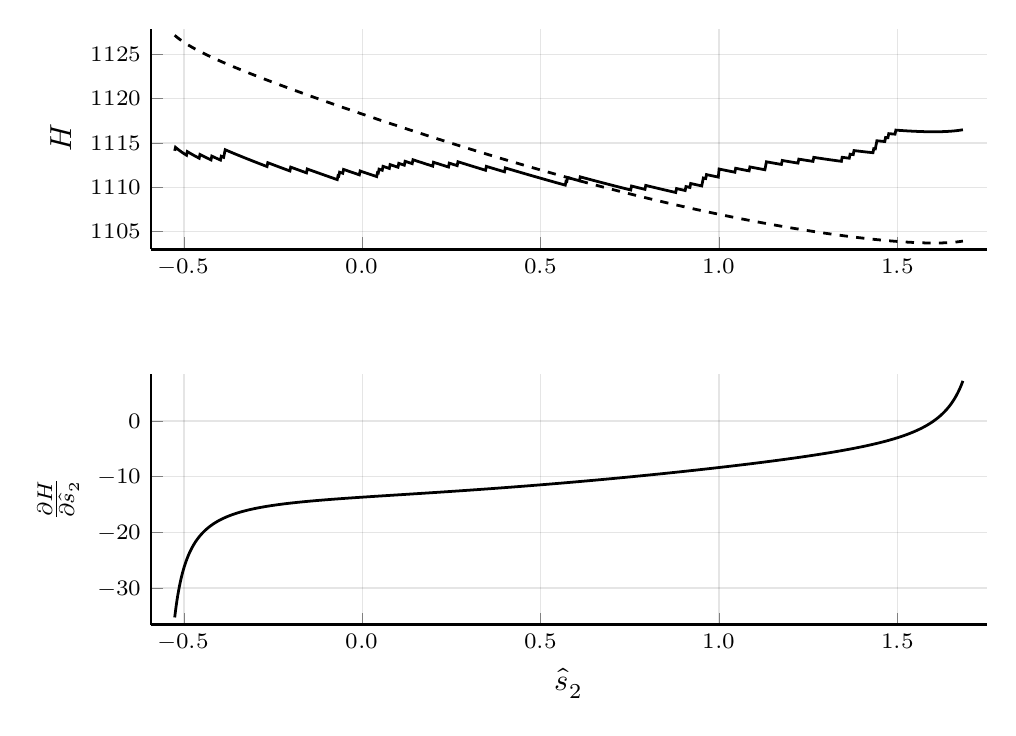
\begin{tikzpicture}[]
\begin{axis}[height = {43.77972222222222mm}, ylabel = {$H$}, xmin = {-0.5918062755323664}, xmax = {1.749891499548597}, ymax = {1127.8598455817862}, xlabel = {}, unbounded coords=jump,scaled x ticks = false,xlabel style = {font = {\fontsize{11 pt}{14.3 pt}\selectfont}, color = {rgb,1:red,0.00000000;green,0.00000000;blue,0.00000000}, draw opacity = 1.0, rotate = 0.0},xmajorgrids = true,xtick = {-0.5,0.0,0.5,1.0,1.5},xticklabels = {$-0.5$,$0.0$,$0.5$,$1.0$,$1.5$},xtick align = inside,xticklabel style = {font = {\fontsize{8 pt}{10.4 pt}\selectfont}, color = {rgb,1:red,0.00000000;green,0.00000000;blue,0.00000000}, draw opacity = 1.0, rotate = 0.0},x grid style = {color = {rgb,1:red,0.00000000;green,0.00000000;blue,0.00000000},
draw opacity = 0.1,
line width = 0.5,
solid},axis lines* = left,x axis line style = {color = {rgb,1:red,0.00000000;green,0.00000000;blue,0.00000000},
draw opacity = 1.0,
line width = 1,
solid},scaled y ticks = false,ylabel style = {font = {\fontsize{11 pt}{14.3 pt}\selectfont}, color = {rgb,1:red,0.00000000;green,0.00000000;blue,0.00000000}, draw opacity = 1.0, rotate = 0.0},ymajorgrids = true,ytick = {1105.0,1110.0,1115.0,1120.0,1125.0},yticklabels = {$1105$,$1110$,$1115$,$1120$,$1125$},ytick align = inside,yticklabel style = {font = {\fontsize{8 pt}{10.4 pt}\selectfont}, color = {rgb,1:red,0.00000000;green,0.00000000;blue,0.00000000}, draw opacity = 1.0, rotate = 0.0},y grid style = {color = {rgb,1:red,0.00000000;green,0.00000000;blue,0.00000000},
draw opacity = 0.1,
line width = 0.5,
solid},axis lines* = left,y axis line style = {color = {rgb,1:red,0.00000000;green,0.00000000;blue,0.00000000},
draw opacity = 1.0,
line width = 1,
solid},    xshift = 0.0mm,
    yshift = 47.66mm,
    axis background/.style={fill={rgb,1:red,1.00000000;green,1.00000000;blue,1.00000000}}
,legend style = {color = {rgb,1:red,0.00000000;green,0.00000000;blue,0.00000000},
draw opacity = 1.0,
line width = 1,
solid,fill = {rgb,1:red,1.00000000;green,1.00000000;blue,1.00000000},font = {\fontsize{8 pt}{10.4 pt}\selectfont}}, ymin = {1103.0022926733182}, width = {121.92mm}]\addplot+ [color = {rgb,1:red,0.00000000;green,0.00000000;blue,0.00000000},
draw opacity = 1.0,
line width = 1,
solid,mark = none,
mark size = 2.0,
mark options = {
    color = {rgb,1:red,0.00000000;green,0.00000000;blue,0.00000000}, draw opacity = 1.0,
    fill = {rgb,1:red,0.00000000;green,0.60560316;blue,0.97868012}, fill opacity = 1.0,
    line width = 1,
    rotate = 0,
    solid
}]coordinates {
(-0.5255318101998864, 1114.118216480952)
(-0.5233204499952657, 1114.506191380215)
(-0.5211090897906451, 1114.431941977204)
(-0.5188977295860245, 1114.3599222478583)
(-0.5166863693814039, 1114.2899343307413)
(-0.5144750091767832, 1114.2218054939783)
(-0.5122636489721626, 1114.1553840532051)
(-0.510052288767542, 1114.0905360861395)
(-0.5078409285629214, 1114.0271427641999)
(-0.5056295683583008, 1113.96509816713)
(-0.5034182081536801, 1113.9043074793663)
(-0.5012068479490596, 1113.8446854908211)
(-0.49899548774443886, 1113.7861553424398)
(-0.49678412753981827, 1113.7286474700811)
(-0.4945727673351976, 1113.672098710251)
(-0.492361407130577, 1113.6164515388068)
(-0.4901500469259564, 1114.0263355088464)
(-0.4879386867213358, 1113.9723383337143)
(-0.48572732651671513, 1113.9190979390419)
(-0.48351596631209454, 1113.8665736864382)
(-0.4813046061074739, 1113.8147280977503)
(-0.4790932459028533, 1113.7635265361146)
(-0.47688188569823264, 1113.712936926258)
(-0.474670525493612, 1113.6629295083935)
(-0.4724591652889914, 1113.613476620981)
(-0.47024780508437075, 1113.5645525083808)
(-0.46803644487975016, 1113.5161331500608)
(-0.4658250846751295, 1113.4681961085114)
(-0.4636137244705089, 1113.4207203934732)
(-0.46140236426588827, 1113.3736863404138)
(-0.45919100406126767, 1113.3270755015)
(-0.456979643856647, 1113.2808705475527)
(-0.45476828365202643, 1113.6997372689448)
(-0.4525569234474058, 1113.6542961387556)
(-0.4503455632427852, 1113.6092147761053)
(-0.44813420303816454, 1113.5644795236246)
(-0.4459228428335439, 1113.5200774772165)
(-0.4437114826289233, 1113.4759964319067)
(-0.44150012242430264, 1113.432224832473)
(-0.43928876221968205, 1113.3887517283588)
(-0.4370774020150614, 1113.3455667324324)
(-0.4348660418104408, 1113.3026599832015)
(-0.43265468160582016, 1113.260022110146)
(-0.43044332140119956, 1113.217644201861)
(-0.4282319611965789, 1113.1755177767448)
(-0.4260206009919583, 1113.1336347559884)
(-0.42380924078733767, 1113.0919874386552)
(-0.421597880582717, 1113.5152505679196)
(-0.41938652037809643, 1113.474052952732)
(-0.4171751601734758, 1113.433069983658)
(-0.4149637999688552, 1113.3922952575558)
(-0.41275243976423454, 1113.351722649863)
(-0.41054107955961394, 1113.3113462988288)
(-0.4083297193549933, 1113.2711605908448)
(-0.4061183591503727, 1113.231160146785)
(-0.40390699894575205, 1113.1913398092731)
(-0.40169563874113146, 1113.1516946308059)
(-0.3994842785365108, 1113.1122198626574)
(-0.39727291833189016, 1113.0729109445094)
(-0.39506155812726956, 1113.4984455840097)
(-0.3928501979226489, 1113.4594553906472)
(-0.3906388377180283, 1113.4206184027955)
(-0.38842747751340767, 1113.381930722688)
(-0.3862161173087871, 1113.808070687437)
(-0.3840047571041664, 1114.234352594214)
(-0.38179339689954583, 1114.1960908721435)
(-0.3795820366949252, 1114.1579642545905)
(-0.3773706764903046, 1114.1199695055154)
(-0.37515931628568394, 1114.0821035032027)
(-0.3729479560810633, 1114.0443632350466)
(-0.3707365958764427, 1114.0067457926327)
(-0.36852523567182205, 1113.9692483670917)
(-0.36631387546720146, 1113.9318682447101)
(-0.3641025152625808, 1113.894602802781)
(-0.3618911550579602, 1113.8574495056773)
(-0.35967979485333956, 1113.8204059011373)
(-0.35746843464871897, 1113.7834696167424)
(-0.3552570744440983, 1113.7466383565832)
(-0.3530457142394777, 1113.709909898095)
(-0.3508343540348571, 1113.6732820890572)
(-0.3486229938302365, 1113.636752844744)
(-0.34641163362561583, 1113.6003201452174)
(-0.3442002734209952, 1113.5639820327563)
(-0.3419889132163746, 1113.5277366094099)
(-0.33977755301175394, 1113.491582034673)
(-0.33756619280713335, 1113.4555165232707)
(-0.3353548326025127, 1113.4195383430513)
(-0.3331434723978921, 1113.3836458129756)
(-0.33093211219327145, 1113.3478373012051)
(-0.32872075198865086, 1113.3121112232752)
(-0.3265093917840302, 1113.2764660403539)
(-0.3242980315794096, 1113.2409002575798)
(-0.32208667137478897, 1113.2054124224749)
(-0.3198753111701683, 1113.1700011234284)
(-0.3176639509655477, 1113.1346649882496)
(-0.3154525907609271, 1113.0994026827805)
(-0.3132412305563065, 1113.0642129095734)
(-0.31102987035168583, 1113.0290944066223)
(-0.30881851014706524, 1112.9940459461502)
(-0.3066071499424446, 1112.959066333448)
(-0.304395789737824, 1112.924154405761)
(-0.30218442953320335, 1112.8893090312247)
(-0.29997306932858275, 1112.8545291078399)
(-0.2977617091239621, 1112.819813562495)
(-0.29555034891934145, 1112.7851613500268)
(-0.29333898871472086, 1112.7505714523152)
(-0.2911276285101002, 1112.7160428774203)
(-0.2889162683054796, 1112.6815746587497)
(-0.28670490810085897, 1112.6471658542605)
(-0.2844935478962384, 1112.6128155456909)
(-0.2822821876916177, 1112.5785228378236)
(-0.28007082748699713, 1112.5442868577768)
(-0.2778594672823765, 1112.5101067543212)
(-0.2756481070777559, 1112.4759816972248)
(-0.27343674687313524, 1112.4419108766213)
(-0.2712253866685146, 1112.4078935024015)
(-0.269014026463894, 1112.3739288036293)
(-0.26680266625927335, 1112.340016027977)
(-0.26459130605465275, 1112.7708365304427)
(-0.2623799458500321, 1112.7370254157875)
(-0.2601685856454115, 1112.7032640735886)
(-0.25795722544079086, 1112.6695518207162)
(-0.25574586523617027, 1112.635887990121)
(-0.2535345050315496, 1112.6022719303846)
(-0.251323144826929, 1112.5687030052798)
(-0.24911178462230837, 1112.5351805933512)
(-0.24690042441768775, 1112.5017040875064)
(-0.24468906421306713, 1112.4682728946245)
(-0.2424777040084465, 1112.434886435175)
(-0.2402663438038259, 1112.4015441428514)
(-0.23805498359920527, 1112.3682454642176)
(-0.23584362339458464, 1112.3349898583626)
(-0.23363226318996402, 1112.3017767965716)
(-0.23142090298534337, 1112.2686057620053)
(-0.22920954278072275, 1112.2354762493876)
(-0.22699818257610213, 1112.2023877647084)
(-0.2247868223714815, 1112.1693398249317)
(-0.2225754621668609, 1112.1363319577156)
(-0.22036410196224027, 1112.1033637011392)
(-0.21815274175761964, 1112.0704346034404)
(-0.21594138155299902, 1112.0375442227598)
(-0.2137300213483784, 1112.004692126894)
(-0.21151866114375778, 1111.9718778930571)
(-0.20930730093913716, 1111.939101107646)
(-0.2070959407345165, 1111.9063613660178)
(-0.2048845805298959, 1111.873658272271)
(-0.20267322032527527, 1111.8409914390343)
(-0.20046186012065464, 1112.2730425765199)
(-0.19825049991603402, 1112.2404471352872)
(-0.1960391397114134, 1112.2078868416077)
(-0.19382777950679278, 1112.1753613402375)
(-0.19161641930217216, 1112.1428702834964)
(-0.18940505909755154, 1112.1104133310912)
(-0.18719369889293092, 1112.0779901499445)
(-0.1849823386883103, 1112.0456004140265)
(-0.18277097848368967, 1112.0132438041962)
(-0.18055961827906902, 1111.9809200080413)
(-0.1783482580744484, 1111.9486287197274)
(-0.17613689786982778, 1111.9163696398498)
(-0.17392553766520716, 1111.8841424752877)
(-0.17171417746058654, 1111.851946939066)
(-0.16950281725596592, 1111.819782750217)
(-0.1672914570513453, 1111.78764963365)
(-0.16508009684672467, 1111.755547320021)
(-0.16286873664210405, 1111.7234755456075)
(-0.16065737643748343, 1111.6914340521862)
(-0.1584460162328628, 1111.6594225869162)
(-0.15623465602824216, 1111.6274409022208)
(-0.15402329582362154, 1112.060170844937)
(-0.15181193561900092, 1112.0282479991652)
(-0.1496005754143803, 1111.9963542217229)
(-0.14738921520975967, 1111.9644892850008)
(-0.14517785500513905, 1111.9326529661212)
(-0.14296649480051843, 1111.9008450468411)
(-0.1407551345958978, 1111.8690653134547)
(-0.13854377439127719, 1111.8373135567003)
(-0.13633241418665656, 1111.8055895716707)
(-0.13412105398203594, 1111.7738931577212)
(-0.1319096937774153, 1111.7422241183872)
(-0.12969833357279467, 1111.7105822612962)
(-0.12748697336817405, 1111.678967398088)
(-0.12527561316355343, 1111.6473793443336)
(-0.12306425295893281, 1111.6158179194563)
(-0.12085289275431219, 1111.5842829466571)
(-0.11864153254969156, 1111.552774252839)
(-0.11643017234507094, 1111.5212916685346)
(-0.11421881214045032, 1111.489835027835)
(-0.11200745193582969, 1111.4584041683222)
(-0.10979609173120906, 1111.4269989309996)
(-0.10758473152658844, 1111.395619160227)
(-0.10537337132196782, 1111.3642647036565)
(-0.1031620111173472, 1111.3329354121702)
(-0.10095065091272658, 1111.301631139817)
(-0.09873929070810594, 1111.2703517437544)
(-0.09652793050348532, 1111.2390970841902)
(-0.0943165702988647, 1111.2078670243238)
(-0.09210521009424408, 1111.1766614302921)
(-0.08989384988962346, 1111.1454801711138)
(-0.08768248968500283, 1111.1143231186363)
(-0.0854711294803822, 1111.0831901474844)
(-0.08325976927576158, 1111.0520811350084)
(-0.08104840907114096, 1111.020995961235)
(-0.07883704886652033, 1110.9899345088184)
(-0.07662568866189971, 1110.9588966629924)
(-0.07441432845727908, 1110.927882311525)
(-0.07220296825265846, 1110.896891344672)
(-0.06999160804803783, 1110.8659236551323)
(-0.06778024784341721, 1111.299661227265)
(-0.06556888763879659, 1111.2687397800075)
(-0.06335752743417597, 1111.7025233916515)
(-0.06114616722955534, 1111.6716477857258)
(-0.05893480702493471, 1111.6407949557727)
(-0.05672344682031409, 1111.6099648082711)
(-0.05451208661569347, 1111.5791572518585)
(-0.05230072641107284, 1112.0130542865527)
(-0.05008936620645222, 1111.9822916466755)
(-0.0478780060018316, 1111.9515513363776)
(-0.04566664579721097, 1111.920833272562)
(-0.04345528559259035, 1111.890137374111)
(-0.041243925387969727, 1111.8594635618517)
(-0.0390325651833491, 1111.8288117585246)
(-0.036821204978728476, 1111.7981818887488)
(-0.034609844774107855, 1111.7675738789924)
(-0.032398484569487226, 1111.7369876575408)
(-0.030187124364866605, 1111.7064231544668)
(-0.02797576416024598, 1111.6758803016003)
(-0.02576440395562536, 1111.6453590324995)
(-0.023553043751004733, 1111.6148592824222)
(-0.02134168354638411, 1111.5843809882979)
(-0.019130323341763483, 1111.5539240886997)
(-0.01691896313714286, 1111.5234885238194)
(-0.014707602932522237, 1111.4930742354388)
(-0.012496242727901613, 1111.462681166905)
(-0.010284882523280988, 1111.4323092631048)
(-0.008073522318660365, 1111.4019584704404)
(-0.005862162114039741, 1111.8363108260635)
(-0.0036508019094191172, 1111.806002100814)
(-0.001439441704798493, 1111.7757143347542)
(0.0007719184998221309, 1111.745447480106)
(0.002983278704442755, 1111.7152014904893)
(0.005194638909063379, 1111.6849763208998)
(0.007405999113684003, 1111.6547719276864)
(0.009617359318304626, 1111.624588268531)
(0.011828719522925251, 1111.594425302426)
(0.014040079727545875, 1111.5642829896556)
(0.0162514399321665, 1111.5341612917746)
(0.01846280013678712, 1111.5040601715887)
(0.020674160341407746, 1111.4739795931341)
(0.02288552054602837, 1111.4439195216617)
(0.025096880750648993, 1111.413879923614)
(0.027308240955269618, 1111.3838607666098)
(0.029519601159890243, 1111.3538620194252)
(0.03173096136451087, 1111.3238836519752)
(0.03394232156913149, 1111.293925635298)
(0.03615368177375211, 1111.2639879415358)
(0.03836504197837274, 1111.234070543919)
(0.04057640218299336, 1111.2041734167508)
(0.04278776238761399, 1111.6389786246484)
(0.04499912259223461, 1111.6091219654904)
(0.04721048279685523, 1112.0439675952168)
(0.04942184300147586, 1112.0141513137387)
(0.05163320320609648, 1111.9843551897386)
(0.053844563410717104, 1111.9545792036183)
(0.05605592361533773, 1111.924823336743)
(0.058267283819958354, 1112.3597696606882)
(0.060478644024578976, 1112.3300539801846)
(0.0626900042291996, 1112.3003583686639)
(0.06490136443382023, 1112.2706828112066)
(0.06711272463844085, 1112.2410272937864)
(0.06932408484306148, 1112.2113918032596)
(0.0715354450476821, 1112.1817763273502)
(0.07374680525230272, 1112.1521808546374)
(0.07595816545692334, 1112.1226053745445)
(0.07816952566154398, 1112.5577319665845)
(0.0803808858661646, 1112.5281964433095)
(0.08259224607078522, 1112.4986808858584)
(0.08480360627540584, 1112.4691852869043)
(0.08701496648002646, 1112.4397096399045)
(0.08922632668464708, 1112.410253939087)
(0.09143768688926772, 1112.3808181794425)
(0.09364904709388834, 1112.3514023567093)
(0.09586040729850896, 1112.3220064673665)
(0.09807176750312958, 1112.2926305086207)
(0.1002831277077502, 1112.2632744783964)
(0.10249448791237083, 1112.698620464585)
(0.10470584811699146, 1112.669304287997)
(0.10691720832161208, 1112.6400080379085)
(0.1091285685262327, 1112.610731715014)
(0.11133992873085333, 1112.5814753206755)
(0.11355128893547395, 1112.5522388569134)
(0.11576264914009458, 1112.5230223263968)
(0.1179740093447152, 1112.493825732435)
(0.12018536954933583, 1112.9293311682268)
(0.12239672975395645, 1112.900174459814)
(0.12460808995857707, 1112.8710377016303)
(0.1268194501631977, 1112.841920899453)
(0.12903081036781833, 1112.8128240596561)
(0.13124217057243895, 1112.7837471891996)
(0.13345353077705957, 1112.7546902956224)
(0.1356648909816802, 1112.7256533870348)
(0.1378762511863008, 1112.6966364721086)
(0.14008761139092143, 1112.6676395600703)
(0.14229897159554206, 1113.1033447499535)
(0.14451033180016268, 1113.0743878735511)
(0.1467216920047833, 1113.0454510309664)
(0.14893305220940395, 1113.0165342335677)
(0.15114441241402457, 1112.9876374932392)
(0.1533557726186452, 1112.958760822374)
(0.1555671328232658, 1112.9299042338687)
(0.15777849302788644, 1112.9010677411136)
(0.15998985323250706, 1112.8722513579878)
(0.16220121343712768, 1112.843455098851)
(0.1644125736417483, 1112.8146789785385)
(0.16662393384636892, 1112.7859230123522)
(0.16883529405098954, 1112.7571872160559)
(0.17104665425561016, 1112.7284716058682)
(0.1732580144602308, 1112.6997761984555)
(0.17546937466485144, 1112.671101010927)
(0.17768073486947206, 1112.642446060827)
(0.17989209507409268, 1112.6138113661304)
(0.1821034552787133, 1112.5851969452356)
(0.18431481548333392, 1112.5566028169578)
(0.18652617568795454, 1112.5280290005253)
(0.18873753589257516, 1112.4994755155717)
(0.19094889609719579, 1112.4709423821316)
(0.1931602563018164, 1112.442429620634)
(0.19537161650643703, 1112.4139372518966)
(0.19758297671105765, 1112.3854652971222)
(0.1997943369156783, 1112.82169586715)
(0.20200569712029892, 1112.7932648054143)
(0.20421705732491954, 1112.7648542234958)
(0.20642841752954016, 1112.7364641440777)
(0.2086397777341608, 1112.7080945902012)
(0.2108511379387814, 1112.6797455852593)
(0.21306249814340203, 1112.6514171529932)
(0.21527385834802265, 1112.6231093174856)
(0.21748521855264327, 1112.594822103157)
(0.2196965787572639, 1112.5665555347616)
(0.22190793896188452, 1112.5383096373807)
(0.22411929916650516, 1112.5100844364197)
(0.2263306593711258, 1112.4818799576024)
(0.2285420195757464, 1112.4536962269667)
(0.23075337978036703, 1112.4255332708613)
(0.23296473998498765, 1112.3973911159394)
(0.23517610018960827, 1112.3692697891559)
(0.2373874603942289, 1112.3411693177613)
(0.23959882059884952, 1112.3130897293004)
(0.24181018080347014, 1112.2850310516042)
(0.24402154100809076, 1112.721675402049)
(0.24623290121271138, 1112.6936586305117)
(0.248444261417332, 1112.6656628549242)
(0.25065562162195265, 1112.6376881042306)
(0.25286698182657324, 1112.6097344076434)
(0.2550783420311939, 1112.581801794639)
(0.2572897022358145, 1112.553890294954)
(0.25950106244043514, 1112.5259999385826)
(0.2617124226450558, 1112.4981307557705)
(0.2639237828496764, 1112.4702827770136)
(0.26613514305429703, 1112.4424560330528)
(0.2683465032589176, 1112.8793326441307)
(0.2705578634635383, 1112.851548462949)
(0.27276922366815887, 1112.8237856102237)
(0.2749805838727795, 1112.7960441176424)
(0.2771919440774001, 1112.76832401712)
(0.27940330428202076, 1112.7406253407974)
(0.28161466448664135, 1112.712948121035)
(0.283826024691262, 1112.6852923904128)
(0.2860373848958826, 1112.6576581817244)
(0.28824874510050325, 1112.630045527975)
(0.2904601053051239, 1112.6024544623785)
(0.2926714655097445, 1112.574885018354)
(0.29488282571436514, 1112.5473372295223)
(0.29709418591898573, 1112.5198111297034)
(0.2993055461236064, 1112.4923067529135)
(0.301516906328227, 1112.4648241333614)
(0.3037282665328476, 1112.437363305446)
(0.3059396267374682, 1112.409924303754)
(0.30815098694208887, 1112.3825071630558)
(0.31036234714670946, 1112.355111918303)
(0.3125737073513301, 1112.3277386046266)
(0.31478506755595076, 1112.300387257333)
(0.31699642776057135, 1112.2730579119022)
(0.319207787965192, 1112.2457506039837)
(0.3214191481698126, 1112.2184653693955)
(0.32363050837443325, 1112.1912022441206)
(0.32584186857905384, 1112.1639612643046)
(0.3280532287836745, 1112.1367424662528)
(0.3302645889882951, 1112.1095458864284)
(0.33247594919291573, 1112.0823715614488)
(0.3346873093975363, 1112.0552195280843)
(0.336898669602157, 1112.0280898232547)
(0.3391100298067776, 1112.0009824840283)
(0.3413213900113982, 1111.9738975476178)
(0.34353275021601887, 1111.9468350513785)
(0.34574411042063946, 1111.919795032807)
(0.3479554706252601, 1112.3574596187973)
(0.3501668308298807, 1112.3304646685997)
(0.35237819103450135, 1112.3034923093785)
(0.35458955123912195, 1112.2765425791683)
(0.3568009114437426, 1112.249615516134)
(0.3590122716483632, 1112.2227111585669)
(0.36122363185298384, 1112.195829544884)
(0.3634349920576045, 1112.1689707136238)
(0.3656463522622251, 1112.1421347034473)
(0.36785771246684573, 1112.1153215531328)
(0.3700690726714663, 1112.0885313015754)
(0.372280432876087, 1112.0617639877853)
(0.37449179308070757, 1112.0350196508853)
(0.3767031532853282, 1112.0082983301083)
(0.3789145134899488, 1111.9816000647966)
(0.38112587369456946, 1111.954924894399)
(0.38333723389919006, 1111.9282728584692)
(0.3855485941038107, 1111.9016439966645)
(0.3877599543084313, 1111.8750383487425)
(0.38997131451305195, 1111.8484559545607)
(0.3921826747176726, 1111.8218968540746)
(0.3943940349222932, 1111.7953610873349)
(0.39660539512691384, 1111.768848694487)
(0.39881675533153443, 1111.7423597157676)
(0.4010281155361551, 1112.180576280765)
(0.4032394757407757, 1112.1541342513772)
(0.4054508359453963, 1112.1277157573677)
(0.4076621961500169, 1112.1013208393267)
(0.40987355635463757, 1112.0749495379282)
(0.41208491655925816, 1112.048601893929)
(0.4142962767638788, 1112.022277948166)
(0.41650763696849946, 1111.9959777415563)
(0.41871899717312006, 1111.9697013150944)
(0.4209303573777407, 1111.9434487098508)
(0.4231417175823613, 1111.917219966971)
(0.42535307778698195, 1111.8910151276743)
(0.42756443799160254, 1111.8648342332501)
(0.4297757981962232, 1111.8386773250606)
(0.4319871584008438, 1111.8125444445348)
(0.43419851860546443, 1111.7864356331704)
(0.43640987881008503, 1111.760350932531)
(0.4386212390147057, 1111.7342903842452)
(0.4408325992193263, 1111.708254030005)
(0.4430439594239469, 1111.6822419115642)
(0.44525531962856757, 1111.6562540707375)
(0.44746667983318816, 1111.6302905494)
(0.4496780400378088, 1111.6043513894836)
(0.4518894002424294, 1111.5784366329785)
(0.45410076044705006, 1111.55254632193)
(0.45631212065167065, 1111.5266804984383)
(0.4585234808562913, 1111.5008392046566)
(0.4607348410609119, 1111.4750224827906)
(0.46294620126553254, 1111.4492303750972)
(0.4651575614701532, 1111.4234629238824)
(0.4673689216747738, 1111.397720171502)
(0.46958028187939443, 1111.3720021603585)
(0.47179164208401503, 1111.3463089329016)
(0.4740030022886357, 1111.3206405316255)
(0.47621436249325627, 1111.2949969990702)
(0.4784257226978769, 1111.2693783778177)
(0.4806370829024975, 1111.2437847104934)
(0.48284844310711816, 1111.2182160397626)
(0.48505980331173876, 1111.1926724083326)
(0.4872711635163594, 1111.1671538589487)
(0.48948252372098, 1111.1416604343951)
(0.49169388392560065, 1111.1161921774933)
(0.4939052441302213, 1111.0907491311011)
(0.4961166043348419, 1111.0653313381122)
(0.49832796453946254, 1111.0399388414542)
(0.5005393247440831, 1111.0145716840896)
(0.5027506849487038, 1110.989229909013)
(0.5049620451533244, 1110.9639135592506)
(0.507173405357945, 1110.9386226778606)
(0.5093847655625656, 1110.9133573079314)
(0.5115961257671863, 1110.8881174925807)
(0.5138074859718069, 1110.8629032749548)
(0.5160188461764276, 1110.8377146982284)
(0.5182302063810481, 1110.8125518056033)
(0.5204415665856688, 1110.7874146403074)
(0.5226529267902894, 1110.7623032455945)
(0.5248642869949101, 1110.7372176647432)
(0.5270756471995306, 1110.7121579410568)
(0.5292870074041512, 1110.6871241178621)
(0.5314983676087719, 1110.6621162385084)
(0.5337097278133925, 1110.6371343463675)
(0.5359210880180131, 1110.6121784848328)
(0.5381324482226337, 1110.587248697319)
(0.5403438084272544, 1110.56234502726)
(0.542555168631875, 1110.5374675181106)
(0.5447665288364957, 1110.5126162133445)
(0.5469778890411162, 1110.4877911564533)
(0.5491892492457369, 1110.4629923909476)
(0.5514006094503575, 1110.4382199603547)
(0.5536119696549782, 1110.4134739082192)
(0.5558233298595987, 1110.3887542781017)
(0.5580346900642194, 1110.3640611135788)
(0.56024605026884, 1110.3393944582433)
(0.5624574104734607, 1110.3147543557018)
(0.5646687706780812, 1110.2901408495757)
(0.5668801308827018, 1110.2655539835002)
(0.5690914910873225, 1110.2409938011251)
(0.5713028512919431, 1110.6811424353718)
(0.5735142114965638, 1110.6566357513962)
(0.5757255717011843, 1111.0968379714045)
(0.577936931905805, 1111.0723849605768)
(0.5801482921104256, 1111.0479588518838)
(0.5823596523150463, 1111.023559689047)
(0.5845710125196668, 1110.9991875157996)
(0.5867823727242875, 1110.9748423758854)
(0.5889937329289081, 1110.9505243130577)
(0.5912050931335288, 1110.9262333710801)
(0.5934164533381494, 1110.9019695937268)
(0.59562781354277, 1110.87773302478)
(0.5978391737473906, 1110.8535237080312)
(0.6000505339520112, 1110.8293416872823)
(0.6022618941566319, 1110.805187006342)
(0.6044732543612524, 1110.7810597090283)
(0.6066846145658731, 1110.756959839168)
(0.6088959747704937, 1110.7328874405948)
(0.6111073349751144, 1111.1735246464102)
(0.6133186951797349, 1111.1495073219457)
(0.6155300553843556, 1111.1255176003178)
(0.6177414155889762, 1111.1015555253916)
(0.6199527757935969, 1111.0776211410391)
(0.6221641359982175, 1111.0537144911402)
(0.624375496202838, 1111.0298356195808)
(0.6265868564074587, 1111.0059845702554)
(0.6287982166120794, 1110.9821613870636)
(0.6310095768167, 1110.9583661139136)
(0.6332209370213205, 1110.93459879472)
(0.6354322972259412, 1110.9108594734032)
(0.6376436574305618, 1110.8871481938922)
(0.6398550176351825, 1110.8634650001218)
(0.642066377839803, 1110.8398099360338)
(0.6442777380444237, 1110.8161830455774)
(0.6464890982490443, 1110.7925843727078)
(0.648700458453665, 1110.7690139613883)
(0.6509118186582856, 1110.7454718555887)
(0.6531231788629062, 1110.7219580992862)
(0.6553345390675268, 1110.6984727364652)
(0.6575458992721475, 1110.6750158111174)
(0.6597572594767681, 1110.6515873672424)
(0.6619686196813886, 1110.6281874488473)
(0.6641799798860093, 1110.604816099947)
(0.66639134009063, 1110.581473364564)
(0.6686027002952506, 1110.5581592867304)
(0.6708140604998712, 1110.534873910485)
(0.6730254207044918, 1110.5116172798764)
(0.6752367809091124, 1110.4883894389618)
(0.6774481411137331, 1110.465190431807)
(0.6796595013183537, 1110.4420203024886)
(0.6818708615229743, 1110.4188790950911)
(0.6840822217275949, 1110.39576685371)
(0.6862935819322156, 1110.3726836224507)
(0.6885049421368362, 1110.3496294454299)
(0.6907163023414568, 1110.3266043667736)
(0.6929276625460774, 1110.3036084306211)
(0.695139022750698, 1110.280641681122)
(0.6973503829553187, 1110.2577041624386)
(0.6995617431599394, 1110.2347959187448)
(0.7017731033645599, 1110.2119169942284)
(0.7039844635691805, 1110.1890674330898)
(0.7061958237738012, 1110.166247279543)
(0.7084071839784218, 1110.1434565778172)
(0.7106185441830424, 1110.120695372155)
(0.712829904387663, 1110.0979637068147)
(0.7150412645922837, 1110.0752616260706)
(0.7172526247969043, 1110.0525891742125)
(0.719463985001525, 1110.0299463955473)
(0.7216753452061455, 1110.0073333343992)
(0.7238867054107662, 1109.9847500351107)
(0.7260980656153868, 1109.9621965420415)
(0.7283094258200075, 1109.9396728995719)
(0.730520786024628, 1109.9171791521007)
(0.7327321462292486, 1109.8947153440474)
(0.7349435064338693, 1109.872281519853)
(0.73715486663849, 1109.849877723979)
(0.7393662268431105, 1109.8275040009107)
(0.7415775870477311, 1109.8051603951553)
(0.7437889472523518, 1109.7828469512442)
(0.7460003074569724, 1109.7605637137335)
(0.7482116676615931, 1109.7383107272042)
(0.7504230278662136, 1109.716088036264)
(0.7526343880708343, 1109.6938956855465)
(0.7548457482754549, 1110.1364158089737)
(0.7570571084800756, 1110.1142842727168)
(0.7592684686846961, 1110.0921832107545)
(0.7614798288893168, 1110.0701126678375)
(0.7636911890939374, 1110.0480726887465)
(0.765902549298558, 1110.026063318295)
(0.7681139095031786, 1110.0040846013292)
(0.7703252697077992, 1109.9821365827286)
(0.7725366299124199, 1109.960219307409)
(0.7747479901170405, 1109.9383328203207)
(0.7769593503216612, 1109.9164771664518)
(0.7791707105262817, 1109.8946523908273)
(0.7813820707309024, 1109.8728585385122)
(0.783593430935523, 1109.8510956546113)
(0.7858047911401437, 1109.8293637842698)
(0.7880161513447642, 1109.8076629726759)
(0.7902275115493849, 1109.7859932650608)
(0.7924388717540055, 1109.7643547067)
(0.7946502319586262, 1110.2074294321746)
(0.7968615921632468, 1110.1858533083337)
(0.7990729523678674, 1110.164308469853)
(0.801284312572488, 1110.142794962198)
(0.8034956727771086, 1110.1213128308848)
(0.8057070329817293, 1110.0998621214815)
(0.8079183931863498, 1110.078442879609)
(0.8101297533909705, 1110.0570551509425)
(0.8123411135955911, 1110.0356989812137)
(0.8145524738002118, 1110.0143744162108)
(0.8167638340048323, 1109.9930815017806)
(0.818975194209453, 1109.9718202838303)
(0.8211865544140736, 1109.9505908083283)
(0.8233979146186943, 1109.9293931213053)
(0.8256092748233149, 1109.9082272688577)
(0.8278206350279355, 1109.8870932971463)
(0.8300319952325561, 1109.8659912524004)
(0.8322433554371768, 1109.8449211809173)
(0.8344547156417974, 1109.823883129066)
(0.836666075846418, 1109.8028771432869)
(0.8388774360510386, 1109.781903270094)
(0.8410887962556592, 1109.7609615560777)
(0.8433001564602799, 1109.740052047905)
(0.8455115166649004, 1109.7191747923218)
(0.8477228768695211, 1109.6983298361547)
(0.8499342370741417, 1109.6775172263128)
(0.8521455972787624, 1109.6567370097894)
(0.854356957483383, 1109.6359892336636)
(0.8565683176880036, 1109.6152739451027)
(0.8587796778926242, 1109.594591191364)
(0.8609910380972449, 1109.573941019796)
(0.8632023983018655, 1109.5533234778413)
(0.865413758506486, 1109.532738613038)
(0.8676251187111067, 1109.5121864730215)
(0.8698364789157274, 1109.4916671055278)
(0.872047839120348, 1109.4711805583934)
(0.8742591993249686, 1109.4507268795599)
(0.8764705595295892, 1109.4303061170738)
(0.8786819197342098, 1109.4099183190908)
(0.8808932799388305, 1109.8542456231357)
(0.8831046401434511, 1109.833923899068)
(0.8853160003480717, 1109.8136352846395)
(0.8875273605526923, 1109.7933798284612)
(0.889738720757313, 1109.7731575792618)
(0.8919500809619336, 1109.7529685858938)
(0.8941614411665542, 1109.732812897332)
(0.8963728013711748, 1109.712690562679)
(0.8985841615757955, 1109.6926016311668)
(0.9007955217804161, 1109.672546152158)
(0.9030068819850368, 1109.6525241751508)
(0.9052182421896573, 1109.632535749779)
(0.907429602394278, 1110.0772630150761)
(0.9096409625988986, 1110.0573418424383)
(0.9118523228035192, 1110.0374543711864)
(0.9140636830081398, 1110.0176006515283)
(0.9162750432127604, 1109.9977807338225)
(0.9184864034173811, 1109.9779946685803)
(0.9206977636220017, 1110.4229245957295)
(0.9229091238266224, 1110.4032063875768)
(0.9251204840312429, 1110.3835221843706)
(0.9273318442358636, 1110.3638720372644)
(0.9295432044404842, 1110.344255997579)
(0.9317545646451049, 1110.3246741168066)
(0.9339659248497254, 1110.3051264466135)
(0.936177285054346, 1110.2856130388434)
(0.9383886452589667, 1110.26613394552)
(0.9406000054635874, 1110.2466892188518)
(0.9428113656682079, 1110.227278911233)
(0.9450227258728285, 1110.207903075249)
(0.9472340860774492, 1110.18856176368)
(0.9494454462820698, 1110.169255029501)
(0.9516568064866905, 1110.1499829258905)
(0.953868166691311, 1110.5954275954891)
(0.9560795268959317, 1111.040907002628)
(0.9582908871005523, 1111.0217391118483)
(0.960502247305173, 1111.0026060664266)
(0.9627136075097935, 1110.9835079205993)
(0.9649249677144142, 1111.4291268180848)
(0.9671363279190348, 1111.41009863505)
(0.9693476881236555, 1111.3911055156718)
(0.971559048328276, 1111.3721475151015)
(0.9737704085328966, 1111.3532246887303)
(0.9759817687375173, 1111.3343370921916)
(0.978193128942138, 1111.3154847813669)
(0.9804044891467586, 1111.2966678123885)
(0.9826158493513791, 1111.2778862416455)
(0.9848272095559998, 1111.2591401257855)
(0.9870385697606204, 1111.240429521723)
(0.9892499299652411, 1111.2217544866398)
(0.9914612901698616, 1111.2031150779924)
(0.9936726503744823, 1111.184511353515)
(0.9958840105791029, 1111.165943371226)
(0.9980953707837236, 1111.1474111894308)
(1.0003067309883442, 1112.058279045247)
(1.0025180911929648, 1112.0398186405318)
(1.0047294513975855, 1112.0213942130038)
(1.006940811602206, 1112.0030058221691)
(1.0091521718068266, 1111.9846535278475)
(1.0113635320114474, 1111.9663373901765)
(1.013574892216068, 1111.9480574696167)
(1.0157862524206884, 1111.929813826959)
(1.0179976126253092, 1111.911606523327)
(1.0202089728299297, 1111.8934356201853)
(1.0224203330345505, 1111.8753011793433)
(1.024631693239171, 1111.8572032629625)
(1.0268430534437916, 1111.839141933561)
(1.0290544136484123, 1111.82111725402)
(1.0312657738530329, 1111.80312928759)
(1.0334771340576536, 1111.7851780978965)
(1.0356884942622742, 1111.7672637489457)
(1.0378998544668947, 1111.7493863051325)
(1.0401112146715155, 1111.731545831245)
(1.042322574876136, 1111.713742392472)
(1.0445339350807565, 1111.6959760544094)
(1.0467452952853773, 1112.1429289723267)
(1.0489566554899978, 1112.1252370341344)
(1.0511680156946186, 1112.1075823959502)
(1.0533793758992391, 1112.0899651250654)
(1.0555907361038597, 1112.0723852892145)
(1.0578020963084804, 1112.0548429565795)
(1.060013456513101, 1112.037338195799)
(1.0622248167177217, 1112.0198710759753)
(1.0644361769223423, 1112.0024416666815)
(1.0666475371269628, 1111.9850500379698)
(1.0688588973315836, 1111.9676962603799)
(1.071070257536204, 1111.9503804049448)
(1.0732816177408246, 1111.933102543201)
(1.0754929779454454, 1111.915862747196)
(1.077704338150066, 1111.8986610894965)
(1.0799156983546867, 1111.8814976431972)
(1.0821270585593072, 1111.864372481929)
(1.0843384187639278, 1111.8472856798683)
(1.0865497789685485, 1112.2949194010046)
(1.088761139173169, 1112.2779095421124)
(1.0909724993777898, 1112.260938268317)
(1.0931838595824104, 1112.2440056560658)
(1.095395219787031, 1112.227111782398)
(1.0976065799916517, 1112.2102567249524)
(1.0998179401962722, 1112.1934405619802)
(1.102029300400893, 1112.176663372352)
(1.1042406606055135, 1112.1599252355697)
(1.106452020810134, 1112.1432262317765)
(1.1086633810147548, 1112.1265664417674)
(1.1108747412193754, 1112.109945947)
(1.1130861014239959, 1112.0933648296045)
(1.1152974616286166, 1112.076823172396)
(1.1175088218332372, 1112.0603210588845)
(1.119720182037858, 1112.0438585732882)
(1.1219315422424785, 1112.0274358005431)
(1.124142902447099, 1112.0110528263162)
(1.1263542626517198, 1111.994709737016)
(1.1285656228563403, 1111.9784066198072)
(1.130776983060961, 1112.4268256518806)
(1.1329883432655816, 1112.8752848326876)
(1.1351997034702022, 1112.8591021624734)
(1.137411063674823, 1112.8429598208065)
(1.1396224238794435, 1112.8268578988177)
(1.141833784084064, 1112.8107964884682)
(1.1440451442886848, 1112.7947756825681)
(1.1462565044933053, 1112.7787955747872)
(1.148467864697926, 1112.762856259671)
(1.1506792249025466, 1112.7469578326547)
(1.1528905851071671, 1112.7311003900784)
(1.155101945311788, 1112.715284029202)
(1.1573133055164084, 1112.6995088482208)
(1.1595246657210292, 1112.6837749462804)
(1.1617360259256497, 1112.6680824234954)
(1.1639473861302703, 1112.6524313809607)
(1.166158746334891, 1112.6368219207736)
(1.1683701065395116, 1112.6212541460468)
(1.170581466744132, 1112.6057281609276)
(1.1727928269487529, 1112.5902440706143)
(1.1750041871533734, 1112.5748019813748)
(1.1772155473579942, 1113.0240840898243)
(1.1794269075626147, 1113.0087263259052)
(1.1816382677672352, 1112.9934108884631)
(1.183849627971856, 1112.9781378882287)
(1.1860609881764765, 1112.9629074370964)
(1.1882723483810973, 1112.947719648145)
(1.1904837085857178, 1112.9325746356567)
(1.1926950687903384, 1112.9174725151383)
(1.1949064289949591, 1112.902413403344)
(1.1971177891995797, 1112.887397418295)
(1.1993291494042002, 1112.872424679302)
(1.201540509608821, 1112.857495306988)
(1.2037518698134415, 1112.8426094233118)
(1.2059632300180623, 1112.8277671515891)
(1.2081745902226828, 1112.8129686165196)
(1.2103859504273033, 1112.7982139442079)
(1.212597310631924, 1112.7835032621906)
(1.2148086708365446, 1112.7688366994605)
(1.2170200310411654, 1112.7542143864932)
(1.219231391245786, 1112.7396364552721)
(1.2214427514504065, 1112.7251030393163)
(1.2236541116550272, 1113.1752963629679)
(1.2258654718596478, 1113.160852384379)
(1.2280768320642685, 1113.146453331102)
(1.230288192268889, 1113.132099343077)
(1.2324995524735096, 1113.1177905619215)
(1.2347109126781304, 1113.103527130963)
(1.236922272882751, 1113.0893091952662)
(1.2391336330873715, 1113.0751369016689)
(1.2413449932919922, 1113.0610103988106)
(1.2435563534966128, 1113.0469298371677)
(1.2457677137012335, 1113.0328953690864)
(1.247979073905854, 1113.0189071488173)
(1.2501904341104746, 1113.0049653325505)
(1.2524017943150954, 1112.9910700784515)
(1.254613154519716, 1112.9772215466971)
(1.2568245147243366, 1112.9634198995145)
(1.2590358749289572, 1112.9496653012188)
(1.2612472351335777, 1112.9359579182515)
(1.2634585953381985, 1112.9222979192211)
(1.265669955542819, 1113.3733675642045)
(1.2678813157474396, 1113.3598028477484)
(1.2700926759520603, 1113.3462860344716)
(1.2723040361566809, 1113.3328173020689)
(1.2745153963613016, 1113.3193968306164)
(1.2767267565659222, 1113.306024802617)
(1.2789381167705427, 1113.2927014030458)
(1.2811494769751635, 1113.2794268194014)
(1.283360837179784, 1113.2662012417497)
(1.2855721973844048, 1113.2530248627793)
(1.2877835575890253, 1113.239897877849)
(1.2899949177936458, 1113.2268204850416)
(1.2922062779982666, 1113.2137928852176)
(1.2944176382028871, 1113.2008152820708)
(1.2966289984075077, 1113.1878878821822)
(1.2988403586121284, 1113.1750108950805)
(1.301051718816749, 1113.1621845332986)
(1.3032630790213697, 1113.149409012436)
(1.3054744392259903, 1113.1366845512193)
(1.3076857994306108, 1113.1240113715658)
(1.3098971596352316, 1113.1113896986487)
(1.312108519839852, 1113.098819760963)
(1.3143198800444729, 1113.0863017903944)
(1.3165312402490934, 1113.0738360222888)
(1.318742600453714, 1113.0614226955229)
(1.3209539606583347, 1113.0490620525795)
(1.3231653208629552, 1113.0367543396208)
(1.3253766810675758, 1113.0244998065666)
(1.3275880412721965, 1113.0122987071725)
(1.329799401476817, 1113.0001512991118)
(1.3320107616814378, 1112.9880578440586)
(1.3342221218860584, 1112.976018607772)
(1.336433482090679, 1112.9640338601846)
(1.3386448422952997, 1112.9521038754922)
(1.3408562024999202, 1112.9402289322459)
(1.343067562704541, 1112.928409313446)
(1.3452789229091615, 1113.3813273959004)
(1.347490283113782, 1113.3696192932834)
(1.3497016433184028, 1113.3579673917977)
(1.3519130035230233, 1113.3463719932402)
(1.354124363727644, 1113.3348334043699)
(1.3563357239322646, 1113.3233519370178)
(1.3585470841368852, 1113.311927908203)
(1.360758444341506, 1113.3005616402472)
(1.3629698045461265, 1113.289253460897)
(1.365181164750747, 1113.2780037034465)
(1.3673925249553678, 1113.731494796124)
(1.3696038851599883, 1113.7203629051853)
(1.371815245364609, 1113.7092904706042)
(1.3740266055692296, 1113.6982778491747)
(1.3762379657738502, 1113.6873254039094)
(1.378449325978471, 1114.141115593449)
(1.3806606861830915, 1114.1302846151718)
(1.3828720463877122, 1114.119514940908)
(1.3850834065923328, 1114.1088069600594)
(1.3872947667969533, 1114.0981610690242)
(1.389506127001574, 1114.0875776713658)
(1.3917174872061946, 1114.0770571779874)
(1.3939288474108151, 1114.06660000731)
(1.396140207615436, 1114.056206585459)
(1.3983515678200564, 1114.0458773464532)
(1.4005629280246772, 1114.035612732402)
(1.4027742882292977, 1114.025413193707)
(1.4049856484339183, 1114.0152791892713)
(1.407197008638539, 1114.0052111867142)
(1.4094083688431596, 1113.9952096625925)
(1.4116197290477803, 1113.9852751026312)
(1.4138310892524009, 1113.9754080019568)
(1.4160424494570214, 1113.965608865344)
(1.4182538096616422, 1113.955878207465)
(1.4204651698662627, 1113.9462165531497)
(1.4226765300708832, 1113.9366244376552)
(1.424887890275504, 1113.9271024069412)
(1.4270992504801245, 1113.9176510179566)
(1.4293106106847453, 1113.9082708389356)
(1.4315219708893658, 1113.8989624497024)
(1.4337333310939864, 1114.3544085312478)
(1.4359446912986071, 1114.3452455090169)
(1.4381560515032277, 1114.336156088804)
(1.4403674117078484, 1114.7918229893237)
(1.442578771912469, 1115.2475647640533)
(1.4447901321170895, 1115.2386999801265)
(1.4470014923217103, 1115.2299113972394)
(1.4492128525263308, 1115.2211997002723)
(1.4514242127309513, 1115.2125655889652)
(1.453635572935572, 1115.2040097783497)
(1.4558469331401926, 1115.1955329991908)
(1.4580582933448134, 1115.1871359984534)
(1.460269653549434, 1115.1788195397787)
(1.4624810137540545, 1115.1705844039825)
(1.4646923739586752, 1115.1624313895684)
(1.4669037341632958, 1115.619043402525)
(1.4691150943679165, 1115.61105709984)
(1.471326454572537, 1115.6031554256356)
(1.4735378147771576, 1115.5953392547267)
(1.4757491749817784, 1116.0522915717636)
(1.477960535186399, 1116.0446491148361)
(1.4801718953910195, 1116.0370949117064)
(1.4823832555956402, 1116.0296299234637)
(1.4845946158002608, 1116.0222551345137)
(1.4868059760048815, 1116.0149715533298)
(1.489017336209502, 1116.007780213241)
(1.4912286964141226, 1116.0006821732477)
(1.4934400566187434, 1115.9936785188743)
(1.4956514168233639, 1116.4514524523156)
(1.4978627770279846, 1116.4446409363209)
(1.5000741372326052, 1116.4379272307167)
(1.5022854974372257, 1116.4313125363722)
(1.5044968576418465, 1116.4247980855046)
(1.506708217846467, 1116.4183851427742)
(1.5089195780510878, 1116.4120750064255)
(1.5111309382557083, 1116.4058690094766)
(1.5133422984603289, 1116.3997685209658)
(1.5155536586649496, 1116.393774947251)
(1.5177650188695702, 1116.3878897333695)
(1.5199763790741907, 1116.382114364461)
(1.5221877392788115, 1116.3764503672542)
(1.524399099483432, 1116.3708993116243)
(1.5266104596880528, 1116.3654628122247)
(1.5288218198926733, 1116.3601425301936)
(1.5310331800972938, 1116.3549401749453)
(1.5332445403019146, 1116.3498575060482)
(1.5354559005065351, 1116.344896335193)
(1.537667260711156, 1116.340058528258)
(1.5398786209157764, 1116.3353460074823)
(1.542089981120397, 1116.330760753742)
(1.5443013413250177, 1116.326304808948)
(1.5465127015296383, 1116.321980278564)
(1.5487240617342588, 1116.3177893342556)
(1.5509354219388796, 1116.3137342166833)
(1.5531467821435, 1116.3098172384362)
(1.5553581423481209, 1116.3060407871305)
(1.5575695025527414, 1116.3024073286717)
(1.559780862757362, 1116.2989194106995)
(1.5619922229619827, 1116.2955796662197)
(1.5642035831666032, 1116.2923908174446)
(1.566414943371224, 1116.2893556798479)
(1.5686263035758445, 1116.286477166454)
(1.570837663780465, 1116.2837582923776)
(1.5730490239850858, 1116.281202179627)
(1.5752603841897064, 1116.2788120621965)
(1.577471744394327, 1116.2765912914647)
(1.5796831045989477, 1116.2745433419186)
(1.5818944648035682, 1116.2726718172357)
(1.584105825008189, 1116.270980456742)
(1.5863171852128095, 1116.2694731422812)
(1.58852854541743, 1116.268153905522)
(1.5907399056220508, 1116.2670269357402)
(1.5929512658266713, 1116.2660965881141)
(1.595162626031292, 1116.2653673925702)
(1.5973739862359126, 1116.2648440632258)
(1.5995853464405332, 1116.2645315084824)
(1.601796706645154, 1116.2644348418137)
(1.6040080668497745, 1116.2645593933162)
(1.606219427054395, 1116.2649107220855)
(1.6084307872590158, 1116.2654946294838)
(1.6106421474636363, 1116.2663171733889)
(1.612853507668257, 1116.267384683499)
(1.6150648678728776, 1116.2687037778028)
(1.6172762280774982, 1116.2702813803098)
(1.619487588282119, 1116.2721247401698)
(1.6216989484867395, 1116.2742414523038)
(1.6239103086913602, 1116.2766394797022)
(1.6261216688959808, 1116.2793271775463)
(1.6283330291006013, 1116.282313319339)
(1.630544389305222, 1116.2856071252495)
(1.6327557495098426, 1116.289218292899)
(1.6349671097144634, 1116.2931570308435)
(1.637178469919084, 1116.2974340950457)
(1.6393898301237044, 1116.3020608286595)
(1.6416011903283252, 1116.3070492054942)
(1.6438125505329457, 1116.3124118775775)
(1.6460239107375663, 1116.3181622272868)
(1.648235270942187, 1116.3243144245873)
(1.6504466311468076, 1116.3308834899897)
(1.6526579913514283, 1116.337885363926)
(1.6548693515560489, 1116.345336983346)
(1.6570807117606694, 1116.3532563664548)
(1.6592920719652902, 1116.361662706654)
(1.6615034321699107, 1116.370576476908)
(1.6637147923745315, 1116.3800195459635)
(1.665926152579152, 1116.3900153080665)
(1.6681375127837725, 1116.4005888281079)
(1.6703488729883933, 1116.4117670044545)
(1.6725602331930138, 1116.4235787521104)
(1.6747715933976344, 1116.4360552093392)
(1.6769829536022551, 1116.4492299714427)
(1.6791943138068757, 1116.4631393561026)
(1.6814056740114964, 1116.4778227055308)
(1.683617034216117, 1116.49332273174)
};
\addplot+ [color = {rgb,1:red,0.00000000;green,0.00000000;blue,0.00000000},
draw opacity = 1.0,
line width = 1,
dashed,mark = none,
mark size = 2.0,
mark options = {
    color = {rgb,1:red,0.00000000;green,0.00000000;blue,0.00000000}, draw opacity = 1.0,
    fill = {rgb,1:red,0.88887350;green,0.43564919;blue,0.27812294}, fill opacity = 1.0,
    line width = 1,
    rotate = 0,
    solid
}]coordinates {
(-0.5255318101998864, 1127.1563299334334)
(-0.5233204499952657, 1127.0783090056186)
(-0.5211090897906451, 1127.002871547078)
(-0.5188977295860245, 1126.9297722879166)
(-0.5166863693814039, 1126.85879919607)
(-0.5144750091767832, 1126.7897677325018)
(-0.5122636489721626, 1126.7225162961533)
(-0.510052288767542, 1126.656902574734)
(-0.5078409285629214, 1126.5928005934436)
(-0.5056295683583008, 1126.5300983073573)
(-0.5034182081536801, 1126.4686956215567)
(-0.5012068479490596, 1126.4085027509466)
(-0.49899548774443886, 1126.34943885214)
(-0.49678412753981827, 1126.2914308749969)
(-0.4945727673351976, 1126.2344125928075)
(-0.492361407130577, 1126.178323778792)
(-0.4901500469259564, 1126.1231095031894)
(-0.4879386867213358, 1126.0687195303592)
(-0.48572732651671513, 1126.015107799285)
(-0.48351596631209454, 1125.9622319740129)
(-0.4813046061074739, 1125.9100530530186)
(-0.4790932459028533, 1125.858535028475)
(-0.47688188569823264, 1125.8076445879587)
(-0.474670525493612, 1125.7573508524083)
(-0.4724591652889914, 1125.707625145171)
(-0.47024780508437075, 1125.6584407878163)
(-0.46803644487975016, 1125.609772919078)
(-0.4658250846751295, 1125.5615983338494)
(-0.4636137244705089, 1125.513895339624)
(-0.46140236426588827, 1125.4666436281643)
(-0.45919100406126767, 1125.4198241604972)
(-0.456979643856647, 1125.3734190636103)
(-0.45476828365202643, 1125.3274115374495)
(-0.4525569234474058, 1125.28178577101)
(-0.4503455632427852, 1125.236526866471)
(-0.44813420303816454, 1125.1916207704712)
(-0.4459228428335439, 1125.147054211728)
(-0.4437114826289233, 1125.1028146443143)
(-0.44150012242430264, 1125.0588901959882)
(-0.43928876221968205, 1125.0152696210403)
(-0.4370774020150614, 1124.9719422572)
(-0.4348660418104408, 1124.9288979861826)
(-0.43265468160582016, 1124.8861271975156)
(-0.43044332140119956, 1124.8436207553254)
(-0.4282319611965789, 1124.801369967795)
(-0.4260206009919583, 1124.7593665590396)
(-0.42380924078733767, 1124.717602643176)
(-0.421597880582717, 1124.6760707003805)
(-0.41938652037809643, 1124.6347635547584)
(-0.4171751601734758, 1124.5936743538607)
(-0.4149637999688552, 1124.552796549703)
(-0.41275243976423454, 1124.512123881158)
(-0.41054107955961394, 1124.471650357603)
(-0.4083297193549933, 1124.431370243716)
(-0.4061183591503727, 1124.3912780453263)
(-0.40390699894575205, 1124.3513684962313)
(-0.40169563874113146, 1124.3116365459036)
(-0.3994842785365108, 1124.2720773480153)
(-0.39727291833189016, 1124.2326862497152)
(-0.39506155812726956, 1124.1934587816022)
(-0.3928501979226489, 1124.1543906483396)
(-0.3906388377180283, 1124.1154777198624)
(-0.38842747751340767, 1124.0767160231333)
(-0.3862161173087871, 1124.0381017344064)
(-0.3840047571041664, 1123.9996311719613)
(-0.38179339689954583, 1123.9613007892756)
(-0.3795820366949252, 1123.923107168602)
(-0.3773706764903046, 1123.8850470149223)
(-0.37515931628568394, 1123.847117150253)
(-0.3729479560810633, 1123.8093145082776)
(-0.3707365958764427, 1123.7716361292823)
(-0.36852523567182205, 1123.734079155378)
(-0.36631387546720146, 1123.6966408259839)
(-0.3641025152625808, 1123.6593184735625)
(-0.3618911550579602, 1123.622109519583)
(-0.35967979485333956, 1123.5850114707039)
(-0.35746843464871897, 1123.5480219151552)
(-0.3552570744440983, 1123.511138519315)
(-0.3530457142394777, 1123.474359024459)
(-0.3508343540348571, 1123.4376812436826)
(-0.3486229938302365, 1123.4011030589745)
(-0.34641163362561583, 1123.3646224184427)
(-0.3442002734209952, 1123.3282373336754)
(-0.3419889132163746, 1123.291945877234)
(-0.33977755301175394, 1123.2557461802687)
(-0.33756619280713335, 1123.2196364302497)
(-0.3353548326025127, 1123.1836148688058)
(-0.3331434723978921, 1123.147679789669)
(-0.33093211219327145, 1123.1118295367116)
(-0.32872075198865086, 1123.0760625020796)
(-0.3265093917840302, 1123.0403771244078)
(-0.3242980315794096, 1123.00477188712)
(-0.32208667137478897, 1122.969245316805)
(-0.3198753111701683, 1122.9337959816655)
(-0.3176639509655477, 1122.8984224900369)
(-0.3154525907609271, 1122.8631234889701)
(-0.3132412305563065, 1122.8278976628785)
(-0.31102987035168583, 1122.792743732242)
(-0.30881851014706524, 1122.7576604523663)
(-0.3066071499424446, 1122.722646612198)
(-0.304395789737824, 1122.6877010331873)
(-0.30218442953320335, 1122.6528225681975)
(-0.29997306932858275, 1122.6180101004638)
(-0.2977617091239621, 1122.5832625425915)
(-0.29555034891934145, 1122.5485788355957)
(-0.29333898871472086, 1122.5139579479824)
(-0.2911276285101002, 1122.4793988748631)
(-0.2889162683054796, 1122.4449006371074)
(-0.28670490810085897, 1122.4104622805276)
(-0.2844935478962384, 1122.3760828750974)
(-0.2822821876916177, 1122.3417615141973)
(-0.28007082748699713, 1122.307497313894)
(-0.2778594672823765, 1122.273289412243)
(-0.2756481070777559, 1122.2391369686213)
(-0.27343674687313524, 1122.2050391630828)
(-0.2712253866685146, 1122.1709951957391)
(-0.269014026463894, 1122.1370042861633)
(-0.26680266625927335, 1122.1030656728158)
(-0.26459130605465275, 1122.0691786124905)
(-0.2623799458500321, 1122.0353423797828)
(-0.2601685856454115, 1122.0015562665742)
(-0.25795722544079086, 1121.9678195815382)
(-0.25574586523617027, 1121.934131649662)
(-0.2535345050315496, 1121.9004918117857)
(-0.251323144826929, 1121.8668994241582)
(-0.24911178462230837, 1121.833353858007)
(-0.24690042441768775, 1121.7998544991253)
(-0.24468906421306713, 1121.7664007474705)
(-0.2424777040084465, 1121.7329920167792)
(-0.2402663438038259, 1121.699627734193)
(-0.23805498359920527, 1121.6663073398986)
(-0.23584362339458464, 1121.6330302867786)
(-0.23363226318996402, 1121.5997960400748)
(-0.23142090298534337, 1121.5666040770623)
(-0.22920954278072275, 1121.5334538867342)
(-0.22699818257610213, 1121.5003449694966)
(-0.2247868223714815, 1121.4672768368744)
(-0.2225754621668609, 1121.4342490112242)
(-0.22036410196224027, 1121.4012610254595)
(-0.21815274175761964, 1121.368312422782)
(-0.21594138155299902, 1121.3354027564228)
(-0.2137300213483784, 1121.302531589391)
(-0.21151866114375778, 1121.2696984942313)
(-0.20930730093913716, 1121.2369030527868)
(-0.2070959407345165, 1121.204144855972)
(-0.2048845805298959, 1121.1714235035504)
(-0.20267322032527527, 1121.13873860392)
(-0.20046186012065464, 1121.1060897739055)
(-0.19825049991603402, 1121.0734766385551)
(-0.1960391397114134, 1121.0408988309455)
(-0.19382777950679278, 1121.0083559919915)
(-0.19161641930217216, 1120.9758477702612)
(-0.18940505909755154, 1120.9433738217967)
(-0.18719369889293092, 1120.910933809941)
(-0.1849823386883103, 1120.8785274051677)
(-0.18277097848368967, 1120.846154284918)
(-0.18055961827906902, 1120.8138141334407)
(-0.1783482580744484, 1120.781506641638)
(-0.17613689786982778, 1120.7492315069148)
(-0.17392553766520716, 1120.7169884330315)
(-0.17171417746058654, 1120.6847771299635)
(-0.16950281725596592, 1120.652597313762)
(-0.1672914570513453, 1120.6204487064194)
(-0.16508009684672467, 1120.5883310357397)
(-0.16286873664210405, 1120.5562440352096)
(-0.16065737643748343, 1120.524187443877)
(-0.1584460162328628, 1120.492161006229)
(-0.15623465602824216, 1120.460164472076)
(-0.15402329582362154, 1120.4281975964366)
(-0.15181193561900092, 1120.3962601394273)
(-0.1496005754143803, 1120.3643518661545)
(-0.14738921520975967, 1120.3324725466096)
(-0.14517785500513905, 1120.3006219555655)
(-0.14296649480051843, 1120.2687998724782)
(-0.1407551345958978, 1120.2370060813892)
(-0.13854377439127719, 1120.2052403708299)
(-0.13633241418665656, 1120.173502533731)
(-0.13412105398203594, 1120.141792367331)
(-0.1319096937774153, 1120.1101096730895)
(-0.12969833357279467, 1120.078454256602)
(-0.12748697336817405, 1120.0468259275156)
(-0.12527561316355343, 1120.0152244994488)
(-0.12306425295893281, 1119.9836497899119)
(-0.12085289275431219, 1119.9521016202293)
(-0.11864153254969156, 1119.9205798154653)
(-0.11643017234507094, 1119.8890842043495)
(-0.11421881214045032, 1119.8576146192058)
(-0.11200745193582969, 1119.8261708958821)
(-0.10979609173120906, 1119.7947528736818)
(-0.10758473152658844, 1119.7633603952977)
(-0.10537337132196782, 1119.7319933067465)
(-0.1031620111173472, 1119.7006514573052)
(-0.10095065091272658, 1119.6693346994493)
(-0.09873929070810594, 1119.6380428887924)
(-0.09652793050348532, 1119.6067758840265)
(-0.0943165702988647, 1119.5755335468648)
(-0.09210521009424408, 1119.5443157419845)
(-0.08989384988962346, 1119.5131223369722)
(-0.08768248968500283, 1119.4819532022698)
(-0.0854711294803822, 1119.4508082111222)
(-0.08325976927576158, 1119.419687239525)
(-0.08104840907114096, 1119.3885901661754)
(-0.07883704886652033, 1119.3575168724215)
(-0.07662568866189971, 1119.3264672422151)
(-0.07441432845727908, 1119.295441162065)
(-0.07220296825265846, 1119.2644385209903)
(-0.06999160804803783, 1119.2334592104762)
(-0.06778024784341721, 1119.2025031244284)
(-0.06556888763879659, 1119.1715701591324)
(-0.06335752743417597, 1119.1406602132095)
(-0.06114616722955534, 1119.1097731875766)
(-0.05893480702493471, 1119.0789089854056)
(-0.05672344682031409, 1119.0480675120841)
(-0.05451208661569347, 1119.0172486751762)
(-0.05230072641107284, 1118.986452384386)
(-0.05008936620645222, 1118.9556785515192)
(-0.0478780060018316, 1118.9249270904477)
(-0.04566664579721097, 1118.8941979170743)
(-0.04345528559259035, 1118.8634909492973)
(-0.041243925387969727, 1118.8328061069774)
(-0.0390325651833491, 1118.8021433119031)
(-0.036821204978728476, 1118.7715024877598)
(-0.034609844774107855, 1118.7408835600966)
(-0.032398484569487226, 1118.710286456295)
(-0.030187124364866605, 1118.6797111055396)
(-0.02797576416024598, 1118.649157438786)
(-0.02576440395562536, 1118.6186253887336)
(-0.023553043751004733, 1118.5881148897945)
(-0.02134168354638411, 1118.5576258780675)
(-0.019130323341763483, 1118.5271582913083)
(-0.01691896313714286, 1118.496712068904)
(-0.014707602932522237, 1118.4662871518449)
(-0.012496242727901613, 1118.4358834827008)
(-0.010284882523280988, 1118.4055010055922)
(-0.008073522318660365, 1118.375139666168)
(-0.005862162114039741, 1118.344799411579)
(-0.0036508019094191172, 1118.3144801904552)
(-0.001439441704798493, 1118.2841819528812)
(0.0007719184998221309, 1118.2539046503728)
(0.002983278704442755, 1118.2236482358549)
(0.005194638909063379, 1118.193412663639)
(0.007405999113684003, 1118.163197889401)
(0.009617359318304626, 1118.1330038701597)
(0.011828719522925251, 1118.1028305642558)
(0.014040079727545875, 1118.072677931331)
(0.0162514399321665, 1118.042545932308)
(0.01846280013678712, 1118.0124345293702)
(0.020674160341407746, 1117.9823436859422)
(0.02288552054602837, 1117.9522733666704)
(0.025096880750648993, 1117.9222235374045)
(0.027308240955269618, 1117.8921941651784)
(0.029519601159890243, 1117.8621852181925)
(0.03173096136451087, 1117.832196665795)
(0.03394232156913149, 1117.8022284784658)
(0.03615368177375211, 1117.7722806277977)
(0.03836504197837274, 1117.7423530864799)
(0.04057640218299336, 1117.7124458282822)
(0.04278776238761399, 1117.682558828037)
(0.04499912259223461, 1117.6526920616247)
(0.04721048279685523, 1117.6228455059577)
(0.04942184300147586, 1117.5930191389637)
(0.05163320320609648, 1117.563212939572)
(0.053844563410717104, 1117.5334268876973)
(0.05605592361533773, 1117.503660964226)
(0.058267283819958354, 1117.473915151)
(0.060478644024578976, 1117.4441894308054)
(0.0626900042291996, 1117.4144837873553)
(0.06490136443382023, 1117.3847982052778)
(0.06711272463844085, 1117.3551326701029)
(0.06932408484306148, 1117.3254871682473)
(0.0715354450476821, 1117.2958616870033)
(0.07374680525230272, 1117.266256214525)
(0.07595816545692334, 1117.2366707398155)
(0.07816952566154398, 1117.2071052527149)
(0.0803808858661646, 1117.177559743888)
(0.08259224607078522, 1117.148034204812)
(0.08480360627540584, 1117.1185286277648)
(0.08701496648002646, 1117.0890430058137)
(0.08922632668464708, 1117.059577332803)
(0.09143768688926772, 1117.0301316033442)
(0.09364904709388834, 1117.0007058128035)
(0.09586040729850896, 1116.9712999572914)
(0.09807176750312958, 1116.9419140336527)
(0.1002831277077502, 1116.9125480394541)
(0.10249448791237083, 1116.883201972976)
(0.10470584811699146, 1116.8538758332006)
(0.10691720832161208, 1116.8245696198028)
(0.1091285685262327, 1116.7952833331397)
(0.11133992873085333, 1116.766016974241)
(0.11355128893547395, 1116.7367705447996)
(0.11576264914009458, 1116.7075440471617)
(0.1179740093447152, 1116.6783374843183)
(0.12018536954933583, 1116.6491508598947)
(0.12239672975395645, 1116.6199841781429)
(0.12460808995857707, 1116.5908374439316)
(0.1268194501631977, 1116.5617106627383)
(0.12903081036781833, 1116.5326038406397)
(0.13124217057243895, 1116.5035169843043)
(0.13345353077705957, 1116.4744501009832)
(0.1356648909816802, 1116.4454031985022)
(0.1378762511863008, 1116.4163762852534)
(0.14008761139092143, 1116.3873693701873)
(0.14229897159554206, 1116.358382462806)
(0.14451033180016268, 1116.3294155731533)
(0.1467216920047833, 1116.3004687118087)
(0.14893305220940395, 1116.271541889879)
(0.15114441241402457, 1116.242635118992)
(0.1533557726186452, 1116.2137484112875)
(0.1555671328232658, 1116.1848817794114)
(0.15777849302788644, 1116.1560352365086)
(0.15998985323250706, 1116.1272087962145)
(0.16220121343712768, 1116.0984024726502)
(0.1644125736417483, 1116.0696162804138)
(0.16662393384636892, 1116.0408502345754)
(0.16883529405098954, 1116.0121043506688)
(0.17104665425561016, 1115.9833786446861)
(0.1732580144602308, 1115.954673133071)
(0.17546937466485144, 1115.9259878327123)
(0.17768073486947206, 1115.897322760938)
(0.17989209507409268, 1115.8686779355087)
(0.1821034552787133, 1115.8400533746114)
(0.18431481548333392, 1115.8114490968546)
(0.18652617568795454, 1115.7828651212608)
(0.18873753589257516, 1115.754301467262)
(0.19094889609719579, 1115.7257581546928)
(0.1931602563018164, 1115.6972352037865)
(0.19537161650643703, 1115.668732635167)
(0.19758297671105765, 1115.640250469846)
(0.1997943369156783, 1115.6117887292148)
(0.20200569712029892, 1115.5833474350413)
(0.20421705732491954, 1115.5549266094638)
(0.20642841752954016, 1115.526526274985)
(0.2086397777341608, 1115.498146454468)
(0.2108511379387814, 1115.4697871711307)
(0.21306249814340203, 1115.4414484485412)
(0.21527385834802265, 1115.4131303106121)
(0.21748521855264327, 1115.384832781596)
(0.2196965787572639, 1115.3565558860812)
(0.22190793896188452, 1115.3282996489854)
(0.22411929916650516, 1115.3000640955536)
(0.2263306593711258, 1115.2718492513507)
(0.2285420195757464, 1115.2436551422586)
(0.23075337978036703, 1115.215481794471)
(0.23296473998498765, 1115.18732923449)
(0.23517610018960827, 1115.15919748912)
(0.2373874603942289, 1115.1310865854646)
(0.23959882059884952, 1115.1029965509222)
(0.24181018080347014, 1115.0749274131808)
(0.24402154100809076, 1115.046879200216)
(0.24623290121271138, 1115.018851940284)
(0.248444261417332, 1114.9908456619203)
(0.25065562162195265, 1114.9628603939332)
(0.25286698182657324, 1114.9348961654018)
(0.2550783420311939, 1114.9069530056713)
(0.2572897022358145, 1114.879030944349)
(0.25950106244043514, 1114.851130011301)
(0.2617124226450558, 1114.8232502366473)
(0.2639237828496764, 1114.7953916507597)
(0.26613514305429703, 1114.7675542842571)
(0.2683465032589176, 1114.7397381680018)
(0.2705578634635383, 1114.711943333097)
(0.27276922366815887, 1114.6841698108813)
(0.2749805838727795, 1114.6564176329275)
(0.2771919440774001, 1114.6286868310376)
(0.27940330428202076, 1114.60097743724)
(0.28161466448664135, 1114.5732894837856)
(0.283826024691262, 1114.5456230031455)
(0.2860373848958826, 1114.5179780280066)
(0.28824874510050325, 1114.4903545912694)
(0.2904601053051239, 1114.4627527260438)
(0.2926714655097445, 1114.4351724656465)
(0.29488282571436514, 1114.4076138435983)
(0.29709418591898573, 1114.3800768936198)
(0.2993055461236064, 1114.35256164963)
(0.301516906328227, 1114.3250681457414)
(0.3037282665328476, 1114.2975964162588)
(0.3059396267374682, 1114.2701464956754)
(0.30815098694208887, 1114.24271841867)
(0.31036234714670946, 1114.2153122201041)
(0.3125737073513301, 1114.1879279350198)
(0.31478506755595076, 1114.160565598636)
(0.31699642776057135, 1114.133225246346)
(0.319207787965192, 1114.1059069137154)
(0.3214191481698126, 1114.0786106364787)
(0.32363050837443325, 1114.0513364505364)
(0.32584186857905384, 1114.0240843919532)
(0.3280532287836745, 1113.9968544969554)
(0.3302645889882951, 1113.9696468019272)
(0.33247594919291573, 1113.9424613434091)
(0.3346873093975363, 1113.9152981580962)
(0.336898669602157, 1113.8881572828334)
(0.3391100298067776, 1113.8610387546155)
(0.3413213900113982, 1113.8339426105829)
(0.34353275021601887, 1113.8068688880203)
(0.34574411042063946, 1113.779817624354)
(0.3479554706252601, 1113.7527888571497)
(0.3501668308298807, 1113.72578262411)
(0.35237819103450135, 1113.6987989630722)
(0.35458955123912195, 1113.6718379120064)
(0.3568009114437426, 1113.6448995090127)
(0.3590122716483632, 1113.6179837923198)
(0.36122363185298384, 1113.5910908002816)
(0.3634349920576045, 1113.5642205713768)
(0.3656463522622251, 1113.5373731442053)
(0.36785771246684573, 1113.5105485574866)
(0.3700690726714663, 1113.4837468500584)
(0.372280432876087, 1113.4569680608736)
(0.37449179308070757, 1113.430212228999)
(0.3767031532853282, 1113.4034793936123)
(0.3789145134899488, 1113.376769594002)
(0.38112587369456946, 1113.350082869564)
(0.38333723389919006, 1113.3234192597993)
(0.3855485941038107, 1113.296778804314)
(0.3877599543084313, 1113.270161542816)
(0.38997131451305195, 1113.243567515113)
(0.3921826747176726, 1113.2169967611117)
(0.3943940349222932, 1113.1904493208158)
(0.39660539512691384, 1113.1639252343232)
(0.39881675533153443, 1113.1374245418258)
(0.4010281155361551, 1113.1109472836063)
(0.4032394757407757, 1113.0844935000378)
(0.4054508359453963, 1113.058063231581)
(0.4076621961500169, 1113.0316565187836)
(0.40987355635463757, 1113.0052734022781)
(0.41208491655925816, 1112.9789139227796)
(0.4142962767638788, 1112.9525781210857)
(0.41650763696849946, 1112.9262660380734)
(0.41871899717312006, 1112.899977714699)
(0.4209303573777407, 1112.8737131919947)
(0.4231417175823613, 1112.8474725110693)
(0.42535307778698195, 1112.8212557131053)
(0.42756443799160254, 1112.7950628393571)
(0.4297757981962232, 1112.7688939311508)
(0.4319871584008438, 1112.7427490298824)
(0.43419851860546443, 1112.7166281770155)
(0.43640987881008503, 1112.690531414081)
(0.4386212390147057, 1112.6644587826752)
(0.4408325992193263, 1112.6384103244584)
(0.4430439594239469, 1112.6123860811535)
(0.44525531962856757, 1112.5863860945458)
(0.44746667983318816, 1112.5604104064796)
(0.4496780400378088, 1112.534459058859)
(0.4518894002424294, 1112.5085320936453)
(0.45410076044705006, 1112.4826295528562)
(0.45631212065167065, 1112.456751478565)
(0.4585234808562913, 1112.4308979128982)
(0.4607348410609119, 1112.405068898036)
(0.46294620126553254, 1112.3792644762093)
(0.4651575614701532, 1112.3534846897)
(0.4673689216747738, 1112.3277295808393)
(0.46958028187939443, 1112.3019991920064)
(0.47179164208401503, 1112.2762935656274)
(0.4740030022886357, 1112.2506127441748)
(0.47621436249325627, 1112.2249567701656)
(0.4784257226978769, 1112.199325686161)
(0.4806370829024975, 1112.1737195347648)
(0.48284844310711816, 1112.1481383586229)
(0.48505980331173876, 1112.1225822004214)
(0.4872711635163594, 1112.097051102887)
(0.48948252372098, 1112.0715451087844)
(0.49169388392560065, 1112.0460642609166)
(0.4939052441302213, 1112.0206086021237)
(0.4961166043348419, 1111.9951781752814)
(0.49832796453946254, 1111.9697730233004)
(0.5005393247440831, 1111.944393189126)
(0.5027506849487038, 1111.9190387157369)
(0.5049620451533244, 1111.8937096461434)
(0.507173405357945, 1111.8684060233884)
(0.5093847655625656, 1111.843127890545)
(0.5115961257671863, 1111.8178752907163)
(0.5138074859718069, 1111.7926482670346)
(0.5160188461764276, 1111.7674468626606)
(0.5182302063810481, 1111.7422711207823)
(0.5204415665856688, 1111.7171210846147)
(0.5226529267902894, 1111.6919967973993)
(0.5248642869949101, 1111.6668983024022)
(0.5270756471995306, 1111.6418256429142)
(0.5292870074041512, 1111.6167788622506)
(0.5314983676087719, 1111.5917580037496)
(0.5337097278133925, 1111.566763110772)
(0.5359210880180131, 1111.5417942267002)
(0.5381324482226337, 1111.5168513949384)
(0.5403438084272544, 1111.491934658911)
(0.542555168631875, 1111.467044062063)
(0.5447665288364957, 1111.442179647858)
(0.5469778890411162, 1111.4173414597792)
(0.5491892492457369, 1111.3925295413278)
(0.5514006094503575, 1111.3677439360224)
(0.5536119696549782, 1111.3429846873994)
(0.5558233298595987, 1111.3182518390113)
(0.5580346900642194, 1111.2935454344272)
(0.56024605026884, 1111.2688655172315)
(0.5624574104734607, 1111.2442121310237)
(0.5646687706780812, 1111.2195853194182)
(0.5668801308827018, 1111.1949851260438)
(0.5690914910873225, 1111.1704115945429)
(0.5713028512919431, 1111.1458647685706)
(0.5735142114965638, 1111.1213446917961)
(0.5757255717011843, 1111.0968514079004)
(0.577936931905805, 1111.0723849605768)
(0.5801482921104256, 1111.0479453935302)
(0.5823596523150463, 1111.0235327504774)
(0.5845710125196668, 1110.9991470751456)
(0.5867823727242875, 1110.9747884112735)
(0.5889937329289081, 1110.9504568026093)
(0.5912050931335288, 1110.9261522929119)
(0.5934164533381494, 1110.9018749259503)
(0.59562781354277, 1110.877624745502)
(0.5978391737473906, 1110.853401795355)
(0.6000505339520112, 1110.8292061193054)
(0.6022618941566319, 1110.8050377611582)
(0.6044732543612524, 1110.7808967647277)
(0.6066846145658731, 1110.7567831738356)
(0.6088959747704937, 1110.7326970323124)
(0.6111073349751144, 1110.708638383996)
(0.6133186951797349, 1110.6846072727328)
(0.6155300553843556, 1110.6606037423765)
(0.6177414155889762, 1110.636627836788)
(0.6199527757935969, 1110.612679599836)
(0.6221641359982175, 1110.5887590753964)
(0.624375496202838, 1110.5648663073523)
(0.6265868564074587, 1110.5410013395935)
(0.6287982166120794, 1110.5171642160176)
(0.6310095768167, 1110.4933549805285)
(0.6332209370213205, 1110.4695736770368)
(0.6354322972259412, 1110.4458203494607)
(0.6376436574305618, 1110.422095041725)
(0.6398550176351825, 1110.3983977977614)
(0.642066377839803, 1110.374728661508)
(0.6442777380444237, 1110.3510876769103)
(0.6464890982490443, 1110.3274748879207)
(0.648700458453665, 1110.3038903384984)
(0.6509118186582856, 1110.28033407261)
(0.6531231788629062, 1110.2568061342288)
(0.6553345390675268, 1110.2333065673356)
(0.6575458992721475, 1110.2098354159186)
(0.6597572594767681, 1110.1863927239735)
(0.6619686196813886, 1110.1629785355033)
(0.6641799798860093, 1110.139592894519)
(0.66639134009063, 1110.1162358450395)
(0.6686027002952506, 1110.092907431092)
(0.6708140604998712, 1110.0696076967117)
(0.6730254207044918, 1110.0463366859426)
(0.6752367809091124, 1110.0230944428374)
(0.6774481411137331, 1109.9998810114578)
(0.6796595013183537, 1109.9766964358746)
(0.6818708615229743, 1109.9535407601682)
(0.6840822217275949, 1109.9304140284287)
(0.6862935819322156, 1109.9073162847567)
(0.6885049421368362, 1109.8842475732629)
(0.6907163023414568, 1109.861207938069)
(0.6929276625460774, 1109.8381974233075)
(0.695139022750698, 1109.8152160731222)
(0.6973503829553187, 1109.7922639316696)
(0.6995617431599394, 1109.7693410431175)
(0.7017731033645599, 1109.7464474516469)
(0.7039844635691805, 1109.7235832014514)
(0.7061958237738012, 1109.7007483367386)
(0.7084071839784218, 1109.6779429017297)
(0.7106185441830424, 1109.6551669406604)
(0.712829904387663, 1109.6324204977814)
(0.7150412645922837, 1109.609703617359)
(0.7172526247969043, 1109.5870163436746)
(0.719463985001525, 1109.564358721027)
(0.7216753452061455, 1109.5417307937319)
(0.7238867054107662, 1109.5191326061217)
(0.7260980656153868, 1109.496564202548)
(0.7283094258200075, 1109.4740256273803)
(0.730520786024628, 1109.4515169250083)
(0.7327321462292486, 1109.429038139841)
(0.7349435064338693, 1109.4065893163086)
(0.73715486663849, 1109.3841704988622)
(0.7393662268431105, 1109.3617817319753)
(0.7415775870477311, 1109.3394230601434)
(0.7437889472523518, 1109.3170945278862)
(0.7460003074569724, 1109.2947961797472)
(0.7482116676615931, 1109.272528060295)
(0.7504230278662136, 1109.2502902141234)
(0.7526343880708343, 1109.2280826858532)
(0.7548457482754549, 1109.2059055201323)
(0.7570571084800756, 1109.1837587616367)
(0.7592684686846961, 1109.1616424550712)
(0.7614798288893168, 1109.1395566451708)
(0.7636911890939374, 1109.1175013767006)
(0.765902549298558, 1109.0954766944578)
(0.7681139095031786, 1109.073482643272)
(0.7703252697077992, 1109.051519268006)
(0.7725366299124199, 1109.029586613557)
(0.7747479901170405, 1109.0076847248583)
(0.7769593503216612, 1108.9858136468786)
(0.7791707105262817, 1108.9639734246243)
(0.7813820707309024, 1108.9421641031406)
(0.783593430935523, 1108.9203857275118)
(0.7858047911401437, 1108.8986383428628)
(0.7880161513447642, 1108.8769219943601)
(0.7902275115493849, 1108.8552367272134)
(0.7924388717540055, 1108.8335825866757)
(0.7946502319586262, 1108.8119596180454)
(0.7968615921632468, 1108.790367866667)
(0.7990729523678674, 1108.768807377933)
(0.801284312572488, 1108.7472781972833)
(0.8034956727771086, 1108.725780370209)
(0.8057070329817293, 1108.7043139422517)
(0.8079183931863498, 1108.6828789590056)
(0.8101297533909705, 1108.661475466119)
(0.8123411135955911, 1108.6401035092947)
(0.8145524738002118, 1108.6187631342925)
(0.8167638340048323, 1108.59745438693)
(0.818975194209453, 1108.5761773130835)
(0.8211865544140736, 1108.5549319586908)
(0.8233979146186943, 1108.533718369751)
(0.8256092748233149, 1108.5125365923277)
(0.8278206350279355, 1108.4913866725492)
(0.8300319952325561, 1108.47026865661)
(0.8322433554371768, 1108.4491825907733)
(0.8344547156417974, 1108.4281285213722)
(0.836666075846418, 1108.4071064948105)
(0.8388774360510386, 1108.386116557566)
(0.8410887962556592, 1108.36515875619)
(0.8433001564602799, 1108.3442331373114)
(0.8455115166649004, 1108.3233397476358)
(0.8477228768695211, 1108.3024786339492)
(0.8499342370741417, 1108.2816498431198)
(0.8521455972787624, 1108.2608534220976)
(0.854356957483383, 1108.2400894179193)
(0.8565683176880036, 1108.2193578777074)
(0.8587796778926242, 1108.1986588486739)
(0.8609910380972449, 1108.1779923781212)
(0.8632023983018655, 1108.157358513445)
(0.865413758506486, 1108.1367573021348)
(0.8676251187111067, 1108.1161887917774)
(0.8698364789157274, 1108.0956530300577)
(0.872047839120348, 1108.0751500647623)
(0.8742591993249686, 1108.0546799437793)
(0.8764705595295892, 1108.034242715103)
(0.8786819197342098, 1108.0138384268334)
(0.8808932799388305, 1107.993467127181)
(0.8831046401434511, 1107.9731288644673)
(0.8853160003480717, 1107.9528236871274)
(0.8875273605526923, 1107.9325516437125)
(0.889738720757313, 1107.9123127828918)
(0.8919500809619336, 1107.892107153456)
(0.8941614411665542, 1107.8719348043178)
(0.8963728013711748, 1107.851795784516)
(0.8985841615757955, 1107.8316901432172)
(0.9007955217804161, 1107.8116179297185)
(0.9030068819850368, 1107.7915791934497)
(0.9052182421896573, 1107.7715739839762)
(0.907429602394278, 1107.7516023510018)
(0.9096409625988986, 1107.7316643443703)
(0.9118523228035192, 1107.71176001407)
(0.9140636830081398, 1107.6918894102344)
(0.9162750432127604, 1107.6720525831468)
(0.9184864034173811, 1107.6522495832412)
(0.9206977636220017, 1107.6324804611072)
(0.9229091238266224, 1107.6127452674912)
(0.9251204840312429, 1107.5930440533)
(0.9273318442358636, 1107.5733768696043)
(0.9295432044404842, 1107.5537437676408)
(0.9317545646451049, 1107.5341447988155)
(0.9339659248497254, 1107.514580014707)
(0.936177285054346, 1107.49504946707)
(0.9383886452589667, 1107.4755532078373)
(0.9406000054635874, 1107.4560912891247)
(0.9428113656682079, 1107.436663763233)
(0.9450227258728285, 1107.4172706826514)
(0.9472340860774492, 1107.3979121000618)
(0.9494454462820698, 1107.3785880683417)
(0.9516568064866905, 1107.3592986405672)
(0.953868166691311, 1107.3400438700176)
(0.9560795268959317, 1107.3208238101774)
(0.9582908871005523, 1107.3016385147425)
(0.960502247305173, 1107.2824880376209)
(0.9627136075097935, 1107.2633724329385)
(0.9649249677144142, 1107.2442917550425)
(0.9671363279190348, 1107.2252460585046)
(0.9693476881236555, 1107.2062353981257)
(0.971559048328276, 1107.18725982894)
(0.9737704085328966, 1107.168319406217)
(0.9759817687375173, 1107.1494141854694)
(0.978193128942138, 1107.1305442224534)
(0.9804044891467586, 1107.1117095731752)
(0.9826158493513791, 1107.0929102938949)
(0.9848272095559998, 1107.07414644113)
(0.9870385697606204, 1107.055418071661)
(0.9892499299652411, 1107.036725242535)
(0.9914612901698616, 1107.0180680110707)
(0.9936726503744823, 1106.9994464348624)
(0.9958840105791029, 1106.9808605717858)
(0.9980953707837236, 1106.9623104800019)
(1.0003067309883442, 1106.9437962179616)
(1.0025180911929648, 1106.9253178444114)
(1.0047294513975855, 1106.906875418398)
(1.006940811602206, 1106.888468999273)
(1.0091521718068266, 1106.8700986466986)
(1.0113635320114474, 1106.8517644206524)
(1.013574892216068, 1106.833466381433)
(1.0157862524206884, 1106.815204589665)
(1.0179976126253092, 1106.7969791063044)
(1.0202089728299297, 1106.778789992645)
(1.0224203330345505, 1106.7606373103224)
(1.024631693239171, 1106.7425211213213)
(1.0268430534437916, 1106.7244414879804)
(1.0290544136484123, 1106.7063984729984)
(1.0312657738530329, 1106.6883921394403)
(1.0334771340576536, 1106.6704225507426)
(1.0356884942622742, 1106.6524897707204)
(1.0378998544668947, 1106.6345938635736)
(1.0401112146715155, 1106.6167348938918)
(1.042322574876136, 1106.5989129266632)
(1.0445339350807565, 1106.5811280272785)
(1.0467452952853773, 1106.5633802615396)
(1.0489566554899978, 1106.5456696956653)
(1.0511680156946186, 1106.527996396298)
(1.0533793758992391, 1106.5103604305118)
(1.0555907361038597, 1106.492761865818)
(1.0578020963084804, 1106.4752007701734)
(1.060013456513101, 1106.4576772119876)
(1.0622248167177217, 1106.4401912601293)
(1.0644361769223423, 1106.4227429839354)
(1.0666475371269628, 1106.405332453217)
(1.0688588973315836, 1106.3879597382688)
(1.071070257536204, 1106.3706249098755)
(1.0732816177408246, 1106.353328039321)
(1.0754929779454454, 1106.3360691983955)
(1.077704338150066, 1106.3188484594052)
(1.0799156983546867, 1106.3016658951792)
(1.0821270585593072, 1106.2845215790785)
(1.0843384187639278, 1106.2674155850054)
(1.0865497789685485, 1106.2503479874117)
(1.088761139173169, 1106.2333188613077)
(1.0909724993777898, 1106.2163282822714)
(1.0931838595824104, 1106.199376326458)
(1.095395219787031, 1106.182463070609)
(1.0976065799916517, 1106.1655885920618)
(1.0998179401962722, 1106.1487529687597)
(1.102029300400893, 1106.131956279262)
(1.1042406606055135, 1106.1151986027535)
(1.106452020810134, 1106.0984800190545)
(1.1086633810147548, 1106.0818006086329)
(1.1108747412193754, 1106.0651604526126)
(1.1130861014239959, 1106.048559632786)
(1.1152974616286166, 1106.0319982316237)
(1.1175088218332372, 1106.0154763322869)
(1.119720182037858, 1105.9989940186374)
(1.1219315422424785, 1105.98255137525)
(1.124142902447099, 1105.9661484874248)
(1.1263542626517198, 1105.9497854411973)
(1.1285656228563403, 1105.933462323352)
(1.130776983060961, 1105.9171792214347)
(1.1329883432655816, 1105.9009362237646)
(1.1351997034702022, 1105.884733419447)
(1.137411063674823, 1105.868570898387)
(1.1396224238794435, 1105.8524487513018)
(1.141833784084064, 1105.8363670697354)
(1.1440451442886848, 1105.8203259460713)
(1.1462565044933053, 1105.8043254735464)
(1.148467864697926, 1105.7883657462667)
(1.1506792249025466, 1105.7724468592198)
(1.1528905851071671, 1105.7565689082905)
(1.155101945311788, 1105.7407319902768)
(1.1573133055164084, 1105.7249362029033)
(1.1595246657210292, 1105.7091816448383)
(1.1617360259256497, 1105.6934684157086)
(1.1639473861302703, 1105.6777966161164)
(1.166158746334891, 1105.6621663476553)
(1.1683701065395116, 1105.6465777129272)
(1.170581466744132, 1105.6310308155594)
(1.1727928269487529, 1105.6155257602215)
(1.1750041871533734, 1105.6000626526438)
(1.1772155473579942, 1105.584641599635)
(1.1794269075626147, 1105.5692627091005)
(1.1816382677672352, 1105.5539260900605)
(1.183849627971856, 1105.538631852671)
(1.1860609881764765, 1105.5233801082406)
(1.1882723483810973, 1105.508170969253)
(1.1904837085857178, 1105.4930045493843)
(1.1926950687903384, 1105.4778809635266)
(1.1949064289949591, 1105.4628003278065)
(1.1971177891995797, 1105.447762759608)
(1.1993291494042002, 1105.432768377593)
(1.201540509608821, 1105.417817301725)
(1.2037518698134415, 1105.4029096532913)
(1.2059632300180623, 1105.3880455549247)
(1.2081745902226828, 1105.3732251306292)
(1.2103859504273033, 1105.3584485058025)
(1.212597310631924, 1105.3437158072613)
(1.2148086708365446, 1105.3290271632663)
(1.2170200310411654, 1105.314382703547)
(1.219231391245786, 1105.2997825593284)
(1.2214427514504065, 1105.2852268633576)
(1.2236541116550272, 1105.27071574993)
(1.2258654718596478, 1105.256249354919)
(1.2280768320642685, 1105.2418278158013)
(1.230288192268889, 1105.227451271688)
(1.2324995524735096, 1105.2131198633535)
(1.2347109126781304, 1105.1988337332648)
(1.236922272882751, 1105.184593025613)
(1.2391336330873715, 1105.1703978863438)
(1.2413449932919922, 1105.1562484631906)
(1.2435563534966128, 1105.1421449057061)
(1.2457677137012335, 1105.1280873652954)
(1.247979073905854, 1105.1140759952516)
(1.2501904341104746, 1105.1001109507886)
(1.2524017943150954, 1105.0861923890782)
(1.254613154519716, 1105.0723204692856)
(1.2568245147243366, 1105.0584953526065)
(1.2590358749289572, 1105.0447172023057)
(1.2612472351335777, 1105.0309861837547)
(1.2634585953381985, 1105.0173024644719)
(1.265669955542819, 1105.003666214163)
(1.2678813157474396, 1104.9900776047627)
(1.2700926759520603, 1104.9765368104768)
(1.2723040361566809, 1104.9630440078242)
(1.2745153963613016, 1104.9495993756834)
(1.2767267565659222, 1104.9362030953357)
(1.2789381167705427, 1104.9228553505127)
(1.2811494769751635, 1104.9095563274427)
(1.283360837179784, 1104.8963062149)
(1.2855721973844048, 1104.8831052042535)
(1.2877835575890253, 1104.869953489518)
(1.2899949177936458, 1104.8568512674055)
(1.2922062779982666, 1104.843798737379)
(1.2944176382028871, 1104.830796101706)
(1.2966289984075077, 1104.8178435655143)
(1.2988403586121284, 1104.8049413368494)
(1.301051718816749, 1104.792089626732)
(1.3032630790213697, 1104.7792886492182)
(1.3054744392259903, 1104.7665386214603)
(1.3076857994306108, 1104.7538397637697)
(1.3098971596352316, 1104.741192299681)
(1.312108519839852, 1104.7285964560167)
(1.3143198800444729, 1104.716052462956)
(1.3165312402490934, 1104.7035605541028)
(1.318742600453714, 1104.6911209665561)
(1.3209539606583347, 1104.6787339409836)
(1.3231653208629552, 1104.6663997216951)
(1.3253766810675758, 1104.6541185567185)
(1.3275880412721965, 1104.641890697878)
(1.329799401476817, 1104.6297164008745)
(1.3320107616814378, 1104.6175959253678)
(1.3342221218860584, 1104.6055295350595)
(1.336433482090679, 1104.5935174977815)
(1.3386448422952997, 1104.5815600855826)
(1.3408562024999202, 1104.5696575748204)
(1.343067562704541, 1104.557810246255)
(1.3452789229091615, 1104.5460183851442)
(1.347490283113782, 1104.5342822813416)
(1.3497016433184028, 1104.522602229399)
(1.3519130035230233, 1104.510978528668)
(1.354124363727644, 1104.4994114834085)
(1.3563357239322646, 1104.4879014028968)
(1.3585470841368852, 1104.476448601539)
(1.360758444341506, 1104.4650533989854)
(1.3629698045461265, 1104.45371612025)
(1.365181164750747, 1104.4424370958318)
(1.3673925249553678, 1104.4312166618413)
(1.3696038851599883, 1104.420055160128)
(1.371815245364609, 1104.408952938414)
(1.3740266055692296, 1104.3979103504296)
(1.3762379657738502, 1104.3869277560543)
(1.378449325978471, 1104.3760055214602)
(1.3806606861830915, 1104.3651440192612)
(1.3828720463877122, 1104.354343628665)
(1.3850834065923328, 1104.3436047356308)
(1.3872947667969533, 1104.3329277330313)
(1.389506127001574, 1104.3223130208182)
(1.3917174872061946, 1104.3117610061956)
(1.3939288474108151, 1104.301272103795)
(1.396140207615436, 1104.2908467358586)
(1.3983515678200564, 1104.2804853324262)
(1.4005629280246772, 1104.2701883315285)
(1.4027742882292977, 1104.259956179387)
(1.4049856484339183, 1104.2497893306188)
(1.407197008638539, 1104.2396882484486)
(1.4094083688431596, 1104.229653404927)
(1.4116197290477803, 1104.2196852811558)
(1.4138310892524009, 1104.209784367521)
(1.4160424494570214, 1104.1999511639322)
(1.4182538096616422, 1104.1901861800695)
(1.4204651698662627, 1104.180489935641)
(1.4226765300708832, 1104.1708629606442)
(1.424887890275504, 1104.1613057956406)
(1.4270992504801245, 1104.1518189920362)
(1.4293106106847453, 1104.142403112372)
(1.4315219708893658, 1104.133058730626)
(1.4337333310939864, 1104.1237864325221)
(1.4359446912986071, 1104.1145868158528)
(1.4381560515032277, 1104.1054604908102)
(1.4403674117078484, 1104.0964080803299)
(1.442578771912469, 1104.0874302204468)
(1.4447901321170895, 1104.0785275606627)
(1.4470014923217103, 1104.0697007643262)
(1.4492128525263308, 1104.0609505090279)
(1.4514242127309513, 1104.052277487008)
(1.453635572935572, 1104.0436824055787)
(1.4558469331401926, 1104.035165987563)
(1.4580582933448134, 1104.0267289717474)
(1.460269653549434, 1104.0183721133535)
(1.4624810137540545, 1104.0100961845255)
(1.4646923739586752, 1104.0019019748356)
(1.4669037341632958, 1103.9937902918098)
(1.4691150943679165, 1103.985761961471)
(1.471326454572537, 1103.977817828907)
(1.4735378147771576, 1103.9699587588543)
(1.4757491749817784, 1103.9621856363106)
(1.477960535186399, 1103.9544993671657)
(1.4801718953910195, 1103.9469008788615)
(1.4823832555956402, 1103.9393911210755)
(1.4845946158002608, 1103.9319710664315)
(1.4868059760048815, 1103.924641711241)
(1.489017336209502, 1103.9174040762716)
(1.4912286964141226, 1103.910259207549)
(1.4934400566187434, 1103.903208177191)
(1.4956514168233639, 1103.896252084276)
(1.4978627770279846, 1103.889392055749)
(1.5000741372326052, 1103.8826292473645)
(1.5022854974372257, 1103.8759648446687)
(1.5044968576418465, 1103.8694000640264)
(1.506708217846467, 1103.8629361536912)
(1.5089195780510878, 1103.8565743949205)
(1.5111309382557083, 1103.8503161031426)
(1.5133422984603289, 1103.8441626291742)
(1.5155536586649496, 1103.8381153604912)
(1.5177650188695702, 1103.8321757225601)
(1.5199763790741907, 1103.8263451802268)
(1.5221877392788115, 1103.820625239172)
(1.524399099483432, 1103.815017447432)
(1.5266104596880528, 1103.8095233969927)
(1.5288218198926733, 1103.8041447254589)
(1.5310331800972938, 1103.7988831178016)
(1.5332445403019146, 1103.7937403081914)
(1.5354559005065351, 1103.7887180819216)
(1.537667260711156, 1103.783818277424)
(1.5398786209157764, 1103.779042788387)
(1.542089981120397, 1103.7743935659785)
(1.5443013413250177, 1103.7698726211831)
(1.5465127015296383, 1103.7654820272571)
(1.5487240617342588, 1103.7612239223124)
(1.5509354219388796, 1103.7571005120353)
(1.5531467821435, 1103.7531140725478)
(1.5553581423481209, 1103.7492669534226)
(1.5575695025527414, 1103.7455615808628)
(1.559780862757362, 1103.7420004610515)
(1.5619922229619827, 1103.7385861836888)
(1.5642035831666032, 1103.7353214257264)
(1.566414943371224, 1103.7322089553127)
(1.5686263035758445, 1103.7292516359612)
(1.570837663780465, 1103.726452430964)
(1.5730490239850858, 1103.723814408058)
(1.5752603841897064, 1103.721340744372)
(1.577471744394327, 1103.7190347316653)
(1.5796831045989477, 1103.716899781888)
(1.5818944648035682, 1103.7149394330786)
(1.584105825008189, 1103.713157355629)
(1.5863171852128095, 1103.7115573589435)
(1.58852854541743, 1103.7101433985224)
(1.5907399056220508, 1103.7089195834994)
(1.5929512658266713, 1103.7078901846749)
(1.595162626031292, 1103.7070596430779)
(1.5973739862359126, 1103.7064325791048)
(1.5995853464405332, 1103.7060138022766)
(1.601796706645154, 1103.705808321671)
(1.6040080668497745, 1103.7058213570822)
(1.606219427054395, 1103.7060583509713)
(1.6084307872590158, 1103.706524981277)
(1.6106421474636363, 1103.7072271751597)
(1.612853507668257, 1103.7081711237624)
(1.6150648678728776, 1103.7093632980827)
(1.6172762280774982, 1103.7108104660533)
(1.619487588282119, 1103.7125197109453)
(1.6216989484867395, 1103.714498451222)
(1.6239103086913602, 1103.7167544619767)
(1.6261216688959808, 1103.7192958981138)
(1.6283330291006013, 1103.7221313194434)
(1.630544389305222, 1103.7252697178817)
(1.6327557495098426, 1103.7287205469775)
(1.6349671097144634, 1103.7324937539997)
(1.637178469919084, 1103.7365998148646)
(1.6393898301237044, 1103.7410497722062)
(1.6416011903283252, 1103.7458552769353)
(1.6438125505329457, 1103.7510286336794)
(1.6460239107375663, 1103.7565828505458)
(1.648235270942187, 1103.7625316937113)
(1.6504466311468076, 1103.768889747411)
(1.6526579913514283, 1103.7756724799804)
(1.6548693515560489, 1103.7828963166987)
(1.6570807117606694, 1103.7905787202915)
(1.6592920719652902, 1103.7987382800804)
(1.6615034321699107, 1103.8073948109172)
(1.6637147923745315, 1103.8165694632223)
(1.665926152579152, 1103.8262848456557)
(1.6681375127837725, 1103.8365651622023)
(1.6703488729883933, 1103.8474363657547)
(1.6725602331930138, 1103.8589263306283)
(1.6747715933976344, 1103.8710650468913)
(1.6769829536022551, 1103.8838848398925)
(1.6791943138068757, 1103.8974206190244)
(1.6814056740114964, 1103.9117101605111)
(1.683617034216117, 1103.9267944299716)
};
\end{axis}
\begin{axis}[height = {47.66027777777777mm}, ylabel = {$\frac{\partial H}{\partial \hat{s}_2}$}, xmin = {-0.5918062755323664}, xmax = {1.749891499548597}, ymax = {8.47526112264902}, xlabel = {$\hat{s}_2$}, unbounded coords=jump,scaled x ticks = false,xlabel style = {font = {\fontsize{11 pt}{14.3 pt}\selectfont}, color = {rgb,1:red,0.00000000;green,0.00000000;blue,0.00000000}, draw opacity = 1.0, rotate = 0.0},xmajorgrids = true,xtick = {-0.5,0.0,0.5,1.0,1.5},xticklabels = {$-0.5$,$0.0$,$0.5$,$1.0$,$1.5$},xtick align = inside,xticklabel style = {font = {\fontsize{8 pt}{10.4 pt}\selectfont}, color = {rgb,1:red,0.00000000;green,0.00000000;blue,0.00000000}, draw opacity = 1.0, rotate = 0.0},x grid style = {color = {rgb,1:red,0.00000000;green,0.00000000;blue,0.00000000},
draw opacity = 0.1,
line width = 0.5,
solid},axis lines* = left,x axis line style = {color = {rgb,1:red,0.00000000;green,0.00000000;blue,0.00000000},
draw opacity = 1.0,
line width = 1,
solid},scaled y ticks = false,ylabel style = {font = {\fontsize{11 pt}{14.3 pt}\selectfont}, color = {rgb,1:red,0.00000000;green,0.00000000;blue,0.00000000}, draw opacity = 1.0, rotate = 0.0},ymajorgrids = true,ytick = {-30.0,-20.0,-10.0,0.0},yticklabels = {$-30$,$-20$,$-10$,$0$},ytick align = inside,yticklabel style = {font = {\fontsize{8 pt}{10.4 pt}\selectfont}, color = {rgb,1:red,0.00000000;green,0.00000000;blue,0.00000000}, draw opacity = 1.0, rotate = 0.0},y grid style = {color = {rgb,1:red,0.00000000;green,0.00000000;blue,0.00000000},
draw opacity = 0.1,
line width = 0.5,
solid},axis lines* = left,y axis line style = {color = {rgb,1:red,0.00000000;green,0.00000000;blue,0.00000000},
draw opacity = 1.0,
line width = 1,
solid},    xshift = 0.0mm,
    yshift = 0.0mm,
    axis background/.style={fill={rgb,1:red,1.00000000;green,1.00000000;blue,1.00000000}}
,legend style = {color = {rgb,1:red,0.00000000;green,0.00000000;blue,0.00000000},
draw opacity = 1.0,
line width = 1,
solid,fill = {rgb,1:red,1.00000000;green,1.00000000;blue,1.00000000},font = {\fontsize{8 pt}{10.4 pt}\selectfont}}, ymin = {-36.55635166582672}, width = {121.92mm}]\addplot+ [color = {rgb,1:red,0.00000000;green,0.00000000;blue,0.00000000},
draw opacity = 1.0,
line width = 1,
solid,mark = none,
mark size = 2.0,
mark options = {
    color = {rgb,1:red,0.00000000;green,0.00000000;blue,0.00000000}, draw opacity = 1.0,
    fill = {rgb,1:red,0.00000000;green,0.60560316;blue,0.97868012}, fill opacity = 1.0,
    line width = 1,
    rotate = 0,
    solid
}]coordinates {
(-0.5255318101998864, -35.28187205860571)
(-0.5233204499952657, -34.113600481237235)
(-0.5211090897906451, -33.05624249210131)
(-0.5188977295860245, -32.094767599675905)
(-0.5166863693814039, -31.216743172033393)
(-0.5144750091767832, -30.411796417310804)
(-0.5122636489721626, -29.671204755502686)
(-0.510052288767542, -28.987580203495583)
(-0.5078409285629214, -28.35462352777246)
(-0.5056295683583008, -27.76693081136978)
(-0.5034182081536801, -27.21983984536556)
(-0.5012068479490596, -26.709307096528)
(-0.49899548774443886, -26.23180837849028)
(-0.49678412753981827, -25.784258064339276)
(-0.4945727673351976, -25.363942924537668)
(-0.492361407130577, -24.96846759167518)
(-0.4901500469259564, -24.595709336131062)
(-0.4879386867213358, -24.243780349346856)
(-0.48572732651671513, -23.910996119810715)
(-0.48351596631209454, -23.595848783613906)
(-0.4813046061074739, -23.296984559964713)
(-0.4790932459028533, -23.01318455933531)
(-0.47688188569823264, -22.74334839042444)
(-0.474670525493612, -22.486480101047675)
(-0.4724591652889914, -22.241676074270693)
(-0.47024780508437075, -22.00811456973081)
(-0.46803644487975016, -21.7850466550377)
(-0.4658250846751295, -21.571788316374647)
(-0.4636137244705089, -21.367713573206423)
(-0.46140236426588827, -21.172248451095626)
(-0.45919100406126767, -20.984865690397708)
(-0.456979643856647, -20.80508008810372)
(-0.45476828365202643, -20.632444386172033)
(-0.4525569234474058, -20.46654563298403)
(-0.4503455632427852, -20.307001955603642)
(-0.44813420303816454, -20.15345968972901)
(-0.4459228428335439, -20.005590821929594)
(-0.4437114826289233, -19.86309070523246)
(-0.44150012242430264, -19.725676014572134)
(-0.43928876221968205, -19.59308291322655)
(-0.4370774020150614, -19.46506540526675)
(-0.4348660418104408, -19.341393852370782)
(-0.43265468160582016, -19.221853636183795)
(-0.43044332140119956, -19.106243949830176)
(-0.4282319611965789, -18.994376704259164)
(-0.4260206009919583, -18.886075536892704)
(-0.42380924078733767, -18.78117491158204)
(-0.421597880582717, -18.67951930020983)
(-0.41938652037809643, -18.580962437426003)
(-0.4171751601734758, -18.4853666410043)
(-0.4149637999688552, -18.392602191176444)
(-0.41275243976423454, -18.30254676305776)
(-0.41054107955961394, -18.21508490694091)
(-0.4083297193549933, -18.130107571812577)
(-0.4061183591503727, -18.047511667956954)
(-0.40390699894575205, -17.967199664955416)
(-0.40169563874113146, -17.889079221785302)
(-0.3994842785365108, -17.813062846066682)
(-0.39727291833189016, -17.73906757981212)
(-0.39506155812726956, -17.66701470930565)
(-0.3928501979226489, -17.596829496976294)
(-0.3906388377180283, -17.52844093334556)
(-0.38842747751340767, -17.461781507316672)
(-0.3862161173087871, -17.396786993242937)
(-0.3840047571041664, -17.33339625336226)
(-0.38179339689954583, -17.27155105431962)
(-0.3795820366949252, -17.21119589661928)
(-0.3773706764903046, -17.152277855955937)
(-0.37515931628568394, -17.094746435470686)
(-0.3729479560810633, -17.03855342806419)
(-0.3707365958764427, -16.98365278797732)
(-0.36852523567182205, -16.930000510919463)
(-0.36631387546720146, -16.877554522088264)
(-0.3641025152625808, -16.826274571481033)
(-0.3618911550579602, -16.77612213595006)
(-0.35967979485333956, -16.72706032750014)
(-0.35746843464871897, -16.679053807369353)
(-0.3552570744440983, -16.6320687054717)
(-0.3530457142394777, -16.586072544815515)
(-0.3508343540348571, -16.54103417054257)
(-0.3486229938302365, -16.496923683261656)
(-0.34641163362561583, -16.453712376376554)
(-0.3442002734209952, -16.41137267713188)
(-0.3419889132163746, -16.369878091121908)
(-0.33977755301175394, -16.32920315002761)
(-0.33756619280713335, -16.289323362364627)
(-0.3353548326025127, -16.25021516704194)
(-0.3331434723978921, -16.211855889545767)
(-0.33093211219327145, -16.17422370057722)
(-0.32872075198865086, -16.13729757698482)
(-0.3265093917840302, -16.101057264844787)
(-0.3242980315794096, -16.065483244552567)
(-0.32208667137478897, -16.03055669779884)
(-0.3198753111701683, -15.996259476312499)
(-0.3176639509655477, -15.962574072261267)
(-0.3154525907609271, -15.929483590208173)
(-0.3132412305563065, -15.896971720529447)
(-0.31102987035168583, -15.865022714205661)
(-0.30881851014706524, -15.833621358904146)
(-0.3066071499424446, -15.802752956275983)
(-0.304395789737824, -15.772403300396496)
(-0.30218442953320335, -15.742558657282377)
(-0.29997306932858275, -15.713205745423329)
(-0.2977617091239621, -15.68433171727009)
(-0.29555034891934145, -15.655924141624467)
(-0.29333898871472086, -15.627970986880493)
(-0.2911276285101002, -15.600460605069113)
(-0.2889162683054796, -15.573381716661855)
(-0.28670490810085897, -15.546723396091583)
(-0.2844935478962384, -15.520475057951284)
(-0.2822821876916177, -15.494626443834097)
(-0.28007082748699713, -15.469167609780028)
(-0.2778594672823765, -15.444088914297051)
(-0.2756481070777559, -15.419381006926145)
(-0.27343674687313524, -15.395034817321678)
(-0.2712253866685146, -15.371041544820157)
(-0.269014026463894, -15.347392648472207)
(-0.26680266625927335, -15.324079837513796)
(-0.26459130605465275, -15.30109506225446)
(-0.2623799458500321, -15.27843050536119)
(-0.2601685856454115, -15.256078573518268)
(-0.25795722544079086, -15.234031889444163)
(-0.25574586523617027, -15.212283284247803)
(-0.2535345050315496, -15.190825790107523)
(-0.251323144826929, -15.169652633256906)
(-0.24911178462230837, -15.148757227262601)
(-0.24690042441768775, -15.12813316658002)
(-0.24468906421306713, -15.107774220373678)
(-0.2424777040084465, -15.087674326589498)
(-0.2402663438038259, -15.067827586267196)
(-0.23805498359920527, -15.04822825808154)
(-0.23584362339458464, -15.028870753101735)
(-0.23363226318996402, -15.009749629758852)
(-0.23142090298534337, -14.99085958901177)
(-0.22920954278072275, -14.972195469702491)
(-0.22699818257610213, -14.953752244092296)
(-0.2247868223714815, -14.935525013570512)
(-0.2225754621668609, -14.917509004528226)
(-0.22036410196224027, -14.899699564389513)
(-0.21815274175761964, -14.882092157793291)
(-0.21594138155299902, -14.86468236291914)
(-0.2137300213483784, -14.847465867950747)
(-0.21151866114375778, -14.830438467671092)
(-0.20930730093913716, -14.813596060183611)
(-0.2070959407345165, -14.79693464375394)
(-0.2048845805298959, -14.780450313767169)
(-0.20267322032527527, -14.76413925979558)
(-0.20046186012065464, -14.747997762772355)
(-0.19825049991603402, -14.732022192266719)
(-0.1960391397114134, -14.7162090038563)
(-0.19382777950679278, -14.700554736592757)
(-0.19161641930217216, -14.685056010556751)
(-0.18940505909755154, -14.669709524498673)
(-0.18719369889293092, -14.65451205356156)
(-0.1849823386883103, -14.639460447082966)
(-0.18277097848368967, -14.624551626472593)
(-0.18055961827906902, -14.609782583162582)
(-0.1783482580744484, -14.595150376627648)
(-0.17613689786982778, -14.580652132472318)
(-0.17392553766520716, -14.566285040582523)
(-0.17171417746058654, -14.552046353339183)
(-0.16950281725596592, -14.53793338389123)
(-0.1672914570513453, -14.523943504485894)
(-0.16508009684672467, -14.510074144853935)
(-0.16286873664210405, -14.496322790647827)
(-0.16065737643748343, -14.482686981930819)
(-0.1584460162328628, -14.46916431171496)
(-0.15623465602824216, -14.455752424546263)
(-0.15402329582362154, -14.44244901513519)
(-0.15181193561900092, -14.429251827030896)
(-0.1496005754143803, -14.416158651337438)
(-0.14738921520975967, -14.40316732547056)
(-0.14517785500513905, -14.390275731953484)
(-0.14296649480051843, -14.377481797250274)
(-0.1407551345958978, -14.36478349063551)
(-0.13854377439127719, -14.352178823098821)
(-0.13633241418665656, -14.33966584628316)
(-0.13412105398203594, -14.327242651455517)
(-0.1319096937774153, -14.314907368508969)
(-0.12969833357279467, -14.302658164994957)
(-0.12748697336817405, -14.290493245184715)
(-0.12527561316355343, -14.278410849158814)
(-0.12306425295893281, -14.266409251923903)
(-0.12085289275431219, -14.254486762555624)
(-0.11864153254969156, -14.242641723366864)
(-0.11643017234507094, -14.230872509100445)
(-0.11421881214045032, -14.219177526145417)
(-0.11200745193582969, -14.207555211776176)
(-0.10979609173120906, -14.196004033413583)
(-0.10758473152658844, -14.184522487907426)
(-0.10537337132196782, -14.17310910083942)
(-0.1031620111173472, -14.16176242584614)
(-0.10095065091272658, -14.150481043961163)
(-0.09873929070810594, -14.139263562975808)
(-0.09652793050348532, -14.12810861681792)
(-0.0943165702988647, -14.117014864947967)
(-0.09210521009424408, -14.105980991772054)
(-0.08989384988962346, -14.095005706071175)
(-0.08768248968500283, -14.084087740446266)
(-0.0854711294803822, -14.073225850778481)
(-0.08325976927576158, -14.062418815704273)
(-0.08104840907114096, -14.051665436104747)
(-0.07883704886652033, -14.040964534608884)
(-0.07662568866189971, -14.03031495511015)
(-0.07441432845727908, -14.019715562296128)
(-0.07220296825265846, -14.009165241190711)
(-0.06999160804803783, -13.998662896708504)
(-0.06778024784341721, -13.988207453221005)
(-0.06556888763879659, -13.977797854134302)
(-0.06335752743417597, -13.967433061477793)
(-0.06114616722955534, -13.957112055503739)
(-0.05893480702493471, -13.94683383429719)
(-0.05672344682031409, -13.936597413396067)
(-0.05451208661569347, -13.926401825421028)
(-0.05230072641107284, -13.916246119714868)
(-0.05008936620645222, -13.906129361991157)
(-0.0478780060018316, -13.8960506339918)
(-0.04566664579721097, -13.886009033153321)
(-0.04345528559259035, -13.876003672281577)
(-0.041243925387969727, -13.86603367923464)
(-0.0390325651833491, -13.856098196613635)
(-0.036821204978728476, -13.84619638146131)
(-0.034609844774107855, -13.836327404968047)
(-0.032398484569487226, -13.826490452185219)
(-0.030187124364866605, -13.81668472174553)
(-0.02797576416024598, -13.806909425590272)
(-0.02576440395562536, -13.797163788703255)
(-0.023553043751004733, -13.787447048851128)
(-0.02134168354638411, -13.7777584563301)
(-0.019130323341763483, -13.768097273718714)
(-0.01691896313714286, -13.758462775636557)
(-0.014707602932522237, -13.748854248508781)
(-0.012496242727901613, -13.739270990336204)
(-0.010284882523280988, -13.729712310470884)
(-0.008073522318660365, -13.720177529396999)
(-0.005862162114039741, -13.710665978516905)
(-0.0036508019094191172, -13.701176999942165)
(-0.001439441704798493, -13.691709946289503)
(0.0007719184998221309, -13.682264180481493)
(0.002983278704442755, -13.672839075551853)
(0.005194638909063379, -13.663434014455273)
(0.007405999113684003, -13.654048389881538)
(0.009617359318304626, -13.644681604074014)
(0.011828719522925251, -13.63533306865218)
(0.014040079727545875, -13.626002204438231)
(0.0162514399321665, -13.616688441287625)
(0.01846280013678712, -13.607391217923407)
(0.020674160341407746, -13.598109981774282)
(0.02288552054602837, -13.588844188816303)
(0.025096880750648993, -13.579593303418081)
(0.027308240955269618, -13.570356798189437)
(0.029519601159890243, -13.5611341538334)
(0.03173096136451087, -13.551924859001451)
(0.03394232156913149, -13.542728410151966)
(0.03615368177375211, -13.53354431141172)
(0.03836504197837274, -13.524372074440457)
(0.04057640218299336, -13.515211218298333)
(0.04278776238761399, -13.506061269316271)
(0.04499912259223461, -13.496921760969073)
(0.04721048279685523, -13.4877922337513)
(0.04942184300147586, -13.478672235055749)
(0.05163320320609648, -13.469561319054531)
(0.053844563410717104, -13.460459046582692)
(0.05605592361533773, -13.451364985024284)
(0.058267283819958354, -13.442278708200798)
(0.060478644024578976, -13.433199796261983)
(0.0626900042291996, -13.424127835578911)
(0.06490136443382023, -13.415062418639296)
(0.06711272463844085, -13.406003143944934)
(0.06932408484306148, -13.39694961591133)
(0.0715354450476821, -13.387901444769314)
(0.07374680525230272, -13.378858246468727)
(0.07595816545692334, -13.369819642584053)
(0.07816952566154398, -13.360785260221968)
(0.0803808858661646, -13.351754731930772)
(0.08259224607078522, -13.342727695611632)
(0.08480360627540584, -13.333703794431637)
(0.08701496648002646, -13.324682676738568)
(0.08922632668464708, -13.315663995977378)
(0.09143768688926772, -13.306647410608347)
(0.09364904709388834, -13.297632584026834)
(0.09586040729850896, -13.288619184484636)
(0.09807176750312958, -13.27960688501288)
(0.1002831277077502, -13.270595363346427)
(0.10249448791237083, -13.261584301849753)
(0.10470584811699146, -13.252573387444285)
(0.10691720832161208, -13.243562311537113)
(0.1091285685262327, -13.234550769951117)
(0.11133992873085333, -13.225538462856402)
(0.11355128893547395, -13.21652509470308)
(0.11576264914009458, -13.207510374155296)
(0.1179740093447152, -13.198494014026563)
(0.12018536954933583, -13.18947573121626)
(0.12239672975395645, -13.180455246647378)
(0.12460808995857707, -13.171432285205416)
(0.1268194501631977, -13.162406575678418)
(0.12903081036781833, -13.15337785069815)
(0.13124217057243895, -13.144345846682338)
(0.13345353077705957, -13.13531030377801)
(0.1356648909816802, -13.126270965805869)
(0.1378762511863008, -13.117227580205682)
(0.14008761139092143, -13.108179897982689)
(0.14229897159554206, -13.099127673654968)
(0.14451033180016268, -13.090070665201772)
(0.1467216920047833, -13.081008634012804)
(0.14893305220940395, -13.07194134483839)
(0.15114441241402457, -13.06286856574057)
(0.1533557726186452, -13.053790068045057)
(0.1555671328232658, -13.044705626294041)
(0.15777849302788644, -13.035615018199847)
(0.15998985323250706, -13.026518024599412)
(0.16220121343712768, -13.01741442940956)
(0.1644125736417483, -13.008304019583083)
(0.16662393384636892, -12.999186585065537)
(0.16883529405098954, -12.990061918752863)
(0.17104665425561016, -12.98092981644969)
(0.1732580144602308, -12.971790076828396)
(0.17546937466485144, -12.962642501388846)
(0.17768073486947206, -12.953486894418841)
(0.17989209507409268, -12.944323062955227)
(0.1821034552787133, -12.935150816745693)
(0.18431481548333392, -12.925969968211193)
(0.18652617568795454, -12.916780332409008)
(0.18873753589257516, -12.907581726996444)
(0.19094889609719579, -12.89837397219512)
(0.1931602563018164, -12.889156890755867)
(0.19537161650643703, -12.879930307924209)
(0.19758297671105765, -12.870694051406403)
(0.1997943369156783, -12.861447951336066)
(0.20200569712029892, -12.852191840241325)
(0.20421705732491954, -12.842925553012515)
(0.20642841752954016, -12.833648926870412)
(0.2086397777341608, -12.824361801334963)
(0.2108511379387814, -12.815064018194544)
(0.21306249814340203, -12.805755421475705)
(0.21527385834802265, -12.796435857413384)
(0.21748521855264327, -12.787105174421633)
(0.2196965787572639, -12.777763223064758)
(0.22190793896188452, -12.768409856028983)
(0.22411929916650516, -12.759044928094506)
(0.2263306593711258, -12.749668296108002)
(0.2285420195757464, -12.740279818955594)
(0.23075337978036703, -12.730879357536205)
(0.23296473998498765, -12.721466774735333)
(0.23517610018960827, -12.712041935399252)
(0.2373874603942289, -12.702604706309565)
(0.23959882059884952, -12.693154956158212)
(0.24181018080347014, -12.683692555522791)
(0.24402154100809076, -12.674217376842313)
(0.24623290121271138, -12.664729294393261)
(0.248444261417332, -12.655228184266077)
(0.25065562162195265, -12.645713924341948)
(0.25286698182657324, -12.636186394269963)
(0.2550783420311939, -12.626645475444613)
(0.2572897022358145, -12.617091050983603)
(0.25950106244043514, -12.607523005706001)
(0.2617124226450558, -12.597941226110724)
(0.2639237828496764, -12.588345600355295)
(0.26613514305429703, -12.578736018234958)
(0.2683465032589176, -12.56911237116206)
(0.2705578634635383, -12.559474552145748)
(0.27276922366815887, -12.54982245577194)
(0.2749805838727795, -12.540155978183583)
(0.2771919440774001, -12.530475017061214)
(0.27940330428202076, -12.520779471603765)
(0.28161466448664135, -12.511069242509652)
(0.283826024691262, -12.501344231958125)
(0.2860373848958826, -12.491604343590888)
(0.28824874510050325, -12.481849482493935)
(0.2904601053051239, -12.472079555179695)
(0.2926714655097445, -12.462294469569361)
(0.29488282571436514, -12.452494134975503)
(0.29709418591898573, -12.442678462084888)
(0.2993055461236064, -12.432847362941557)
(0.301516906328227, -12.423000750930093)
(0.3037282665328476, -12.413138540759158)
(0.3059396267374682, -12.403260648445197)
(0.30815098694208887, -12.393366991296404)
(0.31036234714670946, -12.383457487896854)
(0.3125737073513301, -12.373532058090884)
(0.31478506755595076, -12.363590622967637)
(0.31699642776057135, -12.353633104845835)
(0.319207787965192, -12.343659427258736)
(0.3214191481698126, -12.333669514939261)
(0.32363050837443325, -12.323663293805364)
(0.32584186857905384, -12.313640690945512)
(0.3280532287836745, -12.30360163460441)
(0.3302645889882951, -12.293546054168885)
(0.33247594919291573, -12.283473880153903)
(0.3346873093975363, -12.27338504418883)
(0.336898669602157, -12.263279479003806)
(0.3391100298067776, -12.253157118416288)
(0.3413213900113982, -12.243017897317792)
(0.34353275021601887, -12.232861751660757)
(0.34574411042063946, -12.222688618445572)
(0.3479554706252601, -12.212498435707769)
(0.3501668308298807, -12.20229114250535)
(0.35237819103450135, -12.192066678906285)
(0.35458955123912195, -12.18182498597611)
(0.3568009114437426, -12.17156600576573)
(0.3590122716483632, -12.161289681299307)
(0.36122363185298384, -12.150995956562307)
(0.3634349920576045, -12.140684776489685)
(0.3656463522622251, -12.130356086954187)
(0.36785771246684573, -12.120009834754807)
(0.3700690726714663, -12.10964596760534)
(0.372280432876087, -12.099264434123079)
(0.37449179308070757, -12.088865183817626)
(0.3767031532853282, -12.078448167079847)
(0.3789145134899488, -12.068013335170892)
(0.38112587369456946, -12.05756064021139)
(0.38333723389919006, -12.047090035170717)
(0.3855485941038107, -12.0366014738564)
(0.3877599543084313, -12.026094910903613)
(0.38997131451305195, -12.01557030176479)
(0.3921826747176726, -12.005027602699329)
(0.3943940349222932, -11.994466770763442)
(0.39660539512691384, -11.983887763800036)
(0.39881675533153443, -11.973290540428767)
(0.4010281155361551, -11.962675060036137)
(0.4032394757407757, -11.952041282765713)
(0.4054508359453963, -11.941389169508442)
(0.4076621961500169, -11.93071868189304)
(0.40987355635463757, -11.920029782276492)
(0.41208491655925816, -11.909322433734623)
(0.4142962767638788, -11.898596600052771)
(0.41650763696849946, -11.887852245716537)
(0.41871899717312006, -11.877089335902625)
(0.4209303573777407, -11.866307836469751)
(0.4231417175823613, -11.85550771394965)
(0.42535307778698195, -11.844688935538148)
(0.42756443799160254, -11.833851469086325)
(0.4297757981962232, -11.822995283091736)
(0.4319871584008438, -11.812120346689726)
(0.43419851860546443, -11.801226629644807)
(0.43640987881008503, -11.79031410234211)
(0.4386212390147057, -11.7793827357789)
(0.4408325992193263, -11.768432501556164)
(0.4430439594239469, -11.757463371870287)
(0.44525531962856757, -11.746475319504757)
(0.44746667983318816, -11.735468317821955)
(0.4496780400378088, -11.724442340755012)
(0.4518894002424294, -11.713397362799727)
(0.45410076044705006, -11.702333359006532)
(0.45631212065167065, -11.691250304972526)
(0.4585234808562913, -11.68014817683358)
(0.4607348410609119, -11.66902695125647)
(0.46294620126553254, -11.657886605431095)
(0.4651575614701532, -11.64672711706274)
(0.4673689216747738, -11.63554846436438)
(0.46958028187939443, -11.624350626049043)
(0.47179164208401503, -11.613133581322241)
(0.4740030022886357, -11.601897309874433)
(0.47621436249325627, -11.590641791873539)
(0.4784257226978769, -11.579367007957506)
(0.4806370829024975, -11.568072939226914)
(0.48284844310711816, -11.556759567237654)
(0.48505980331173876, -11.545426873993591)
(0.4872711635163594, -11.534074841939361)
(0.48948252372098, -11.522703453953111)
(0.49169388392560065, -11.511312693339352)
(0.4939052441302213, -11.499902543821833)
(0.4961166043348419, -11.488472989536438)
(0.49832796453946254, -11.477024015024147)
(0.5005393247440831, -11.465555605224004)
(0.5027506849487038, -11.454067745466162)
(0.5049620451533244, -11.44256042146492)
(0.507173405357945, -11.431033619311838)
(0.5093847655625656, -11.419487325468841)
(0.5115961257671863, -11.407921526761388)
(0.5138074859718069, -11.396336210371677)
(0.5160188461764276, -11.384731363831841)
(0.5182302063810481, -11.373106975017226)
(0.5204415665856688, -11.36146303213965)
(0.5226529267902894, -11.349799523740733)
(0.5248642869949101, -11.338116438685221)
(0.5270756471995306, -11.326413766154362)
(0.5292870074041512, -11.31469149563928)
(0.5314983676087719, -11.302949616934415)
(0.5337097278133925, -11.291188120130926)
(0.5359210880180131, -11.279406995610177)
(0.5381324482226337, -11.267606234037235)
(0.5403438084272544, -11.255785826354348)
(0.542555168631875, -11.243945763774473)
(0.5447665288364957, -11.232086037774843)
(0.5469778890411162, -11.220206640090518)
(0.5491892492457369, -11.208307562707974)
(0.5514006094503575, -11.196388797858694)
(0.5536119696549782, -11.184450338012812)
(0.5558233298595987, -11.17249217587272)
(0.5580346900642194, -11.160514304366725)
(0.56024605026884, -11.148516716642709)
(0.5624574104734607, -11.136499406061834)
(0.5646687706780812, -11.12446236619218)
(0.5668801308827018, -11.112405590802497)
(0.5690914910873225, -11.100329073855889)
(0.5713028512919431, -11.08823280950355)
(0.5735142114965638, -11.076116792078475)
(0.5757255717011843, -11.063981016089247)
(0.577936931905805, -11.051825476213734)
(0.5801482921104256, -11.039650167292892)
(0.5823596523150463, -11.0274550843245)
(0.5845710125196668, -11.015240222456933)
(0.5867823727242875, -11.003005576982956)
(0.5889937329289081, -10.990751143333497)
(0.5912050931335288, -10.978476917071408)
(0.5934164533381494, -10.966182893885279)
(0.59562781354277, -10.953869069583215)
(0.5978391737473906, -10.94153544008664)
(0.6000505339520112, -10.929182001424055)
(0.6022618941566319, -10.916808749724863)
(0.6044732543612524, -10.904415681213152)
(0.6066846145658731, -10.89200279220145)
(0.6088959747704937, -10.879570079084582)
(0.6111073349751144, -10.867117538333364)
(0.6133186951797349, -10.85464516648846)
(0.6155300553843556, -10.842152960154108)
(0.6177414155889762, -10.829640915991922)
(0.6199527757935969, -10.817109030714613)
(0.6221641359982175, -10.804557301079816)
(0.624375496202838, -10.791985723883755)
(0.6265868564074587, -10.779394295955045)
(0.6287982166120794, -10.766783014148402)
(0.6310095768167, -10.754151875338371)
(0.6332209370213205, -10.741500876413031)
(0.6354322972259412, -10.728830014267702)
(0.6376436574305618, -10.716139285798619)
(0.6398550176351825, -10.70342868789664)
(0.642066377839803, -10.690698217440872)
(0.6442777380444237, -10.677947871292332)
(0.6464890982490443, -10.665177646287587)
(0.648700458453665, -10.652387539232352)
(0.6509118186582856, -10.639577546895127)
(0.6531231788629062, -10.626747666000725)
(0.6553345390675268, -10.613897893223877)
(0.6575458992721475, -10.601028225182752)
(0.6597572594767681, -10.588138658432513)
(0.6619686196813886, -10.575229189458783)
(0.6641799798860093, -10.562299814671139)
(0.66639134009063, -10.549350530396591)
(0.6686027002952506, -10.536381332872995)
(0.6708140604998712, -10.523392218242474)
(0.6730254207044918, -10.510383182544802)
(0.6752367809091124, -10.497354221710776)
(0.6774481411137331, -10.484305331555527)
(0.6796595013183537, -10.471236507771854)
(0.6818708615229743, -10.458147745923487)
(0.6840822217275949, -10.445039041438344)
(0.6862935819322156, -10.431910389601732)
(0.6885049421368362, -10.41876178554956)
(0.6907163023414568, -10.405593224261477)
(0.6929276625460774, -10.392404700554001)
(0.695139022750698, -10.37919620907361)
(0.6973503829553187, -10.365967744289794)
(0.6995617431599394, -10.35271930048807)
(0.7017731033645599, -10.339450871762969)
(0.7039844635691805, -10.326162452010971)
(0.7061958237738012, -10.312854034923422)
(0.7084071839784218, -10.299525613979398)
(0.7106185441830424, -10.286177182438514)
(0.712829904387663, -10.272808733333731)
(0.7150412645922837, -10.259420259464079)
(0.7172526247969043, -10.24601175338735)
(0.719463985001525, -10.232583207412775)
(0.7216753452061455, -10.219134613593603)
(0.7238867054107662, -10.205665963719678)
(0.7260980656153868, -10.192177249309937)
(0.7283094258200075, -10.17866846160488)
(0.730520786024628, -10.16513959155898)
(0.7327321462292486, -10.151590629833045)
(0.7349435064338693, -10.13802156678652)
(0.73715486663849, -10.12443239246975)
(0.7393662268431105, -10.110823096616166)
(0.7415775870477311, -10.097193668634446)
(0.7437889472523518, -10.083544097600583)
(0.7460003074569724, -10.06987437224992)
(0.7482116676615931, -10.056184480969133)
(0.7504230278662136, -10.042474411788108)
(0.7526343880708343, -10.028744152371797)
(0.7548457482754549, -10.014993690012021)
(0.7570571084800756, -10.001223011619144)
(0.7592684686846961, -9.987432103713774)
(0.7614798288893168, -9.973620952418285)
(0.7636911890939374, -9.959789543448377)
(0.765902549298558, -9.94593786210451)
(0.7681139095031786, -9.93206589326327)
(0.7703252697077992, -9.918173621368641)
(0.7725366299124199, -9.904261030423278)
(0.7747479901170405, -9.890328103979623)
(0.7769593503216612, -9.876374825130966)
(0.7791707105262817, -9.862401176502466)
(0.7813820707309024, -9.848407140242031)
(0.783593430935523, -9.834392698011165)
(0.7858047911401437, -9.820357830975682)
(0.7880161513447642, -9.806302519796418)
(0.7902275115493849, -9.79222674461973)
(0.7924388717540055, -9.778130485068047)
(0.7946502319586262, -9.764013720230196)
(0.7968615921632468, -9.749876428651755)
(0.7990729523678674, -9.735718588325224)
(0.801284312572488, -9.721540176680133)
(0.8034956727771086, -9.707341170573077)
(0.8057070329817293, -9.693121546277599)
(0.8079183931863498, -9.678881279474014)
(0.8101297533909705, -9.664620345239117)
(0.8123411135955911, -9.650338718035755)
(0.8145524738002118, -9.636036371702362)
(0.8167638340048323, -9.62171327944232)
(0.818975194209453, -9.607369413813217)
(0.8211865544140736, -9.593004746716026)
(0.8233979146186943, -9.578619249384142)
(0.8256092748233149, -9.564212892372307)
(0.8278206350279355, -9.5497856455454)
(0.8300319952325561, -9.535337478067142)
(0.8322433554371768, -9.520868358388624)
(0.8344547156417974, -9.506378254236772)
(0.836666075846418, -9.491867132602607)
(0.8388774360510386, -9.477334959729458)
(0.8410887962556592, -9.46278170110095)
(0.8433001564602799, -9.448207321428928)
(0.8455115166649004, -9.43361178464123)
(0.8477228768695211, -9.418995053869253)
(0.8499342370741417, -9.404357091435482)
(0.8521455972787624, -9.389697858840766)
(0.854356957483383, -9.375017316751517)
(0.8565683176880036, -9.360315424986734)
(0.8587796778926242, -9.345592142504847)
(0.8609910380972449, -9.33084742739045)
(0.8632023983018655, -9.316081236840812)
(0.865413758506486, -9.301293527152298)
(0.8676251187111067, -9.28648425370654)
(0.8698364789157274, -9.271653370956512)
(0.872047839120348, -9.256800832412377)
(0.8742591993249686, -9.241926590627186)
(0.8764705595295892, -9.227030597182376)
(0.8786819197342098, -9.212112802673113)
(0.8808932799388305, -9.197173156693419)
(0.8831046401434511, -9.182211607821099)
(0.8853160003480717, -9.167228103602541)
(0.8875273605526923, -9.15222259053723)
(0.889738720757313, -9.137195014062096)
(0.8919500809619336, -9.122145318535694)
(0.8941614411665542, -9.10707344722211)
(0.8963728013711748, -9.091979342274673)
(0.8985841615757955, -9.07686294471951)
(0.9007955217804161, -9.061724194438781)
(0.9030068819850368, -9.046563030153742)
(0.9052182421896573, -9.031379389407583)
(0.907429602394278, -9.016173208548015)
(0.9096409625988986, -9.000944422709605)
(0.9118523228035192, -8.985692965795923)
(0.9140636830081398, -8.970418770461349)
(0.9162750432127604, -8.95512176809272)
(0.9184864034173811, -8.939801888790644)
(0.9206977636220017, -8.924459061350618)
(0.9229091238266224, -8.909093213243814)
(0.9251204840312429, -8.893704270597645)
(0.9273318442358636, -8.878292158176007)
(0.9295432044404842, -8.862856799359271)
(0.9317545646451049, -8.847398116123957)
(0.9339659248497254, -8.831916029022175)
(0.936177285054346, -8.816410457160654)
(0.9383886452589667, -8.80088131817958)
(0.9406000054635874, -8.785328528231036)
(0.9428113656682079, -8.769752001957185)
(0.9450227258728285, -8.754151652468085)
(0.9472340860774492, -8.738527391319185)
(0.9494454462820698, -8.72287912848849)
(0.9516568064866905, -8.707206772353388)
(0.953868166691311, -8.691510229667099)
(0.9560795268959317, -8.675789405534783)
(0.9582908871005523, -8.660044203389278)
(0.960502247305173, -8.644274524966495)
(0.9627136075097935, -8.62848027028036)
(0.9649249677144142, -8.612661337597451)
(0.9671363279190348, -8.59681762341118)
(0.9693476881236555, -8.580949022415608)
(0.971559048328276, -8.565055427478825)
(0.9737704085328966, -8.549136729615913)
(0.9759817687375173, -8.533192817961506)
(0.978193128942138, -8.517223579741875)
(0.9804044891467586, -8.50122890024659)
(0.9826158493513791, -8.48520866279973)
(0.9848272095559998, -8.469162748730614)
(0.9870385697606204, -8.453091037344068)
(0.9892499299652411, -8.4369934058902)
(0.9914612901698616, -8.420869729533706)
(0.9936726503744823, -8.404719881322624)
(0.9958840105791029, -8.38854373215664)
(0.9980953707837236, -8.37234115075481)
(1.0003067309883442, -8.356112003622778)
(1.0025180911929648, -8.339856155019433)
(1.0047294513975855, -8.323573466923042)
(1.006940811602206, -8.307263798996745)
(1.0091521718068266, -8.290927008553558)
(1.0113635320114474, -8.274562950520691)
(1.013574892216068, -8.258171477403343)
(1.0157862524206884, -8.241752439247804)
(1.0179976126253092, -8.225305683603994)
(1.0202089728299297, -8.2088310554873)
(1.0224203330345505, -8.192328397339798)
(1.024631693239171, -8.175797548990754)
(1.0268430534437916, -8.15923834761649)
(1.0290544136484123, -8.142650627699512)
(1.0312657738530329, -8.12603422098693)
(1.0334771340576536, -8.109388956448164)
(1.0356884942622742, -8.092714660231865)
(1.0378998544668947, -8.07601115562209)
(1.0401112146715155, -8.059278262993704)
(1.042322574876136, -8.04251579976701)
(1.0445339350807565, -8.02572358036145)
(1.0467452952853773, -8.00890141614864)
(1.0489566554899978, -7.992049115404388)
(1.0511680156946186, -7.975166483259997)
(1.0533793758992391, -7.958253321652518)
(1.0555907361038597, -7.94130942927424)
(1.0578020963084804, -7.924334601521155)
(1.060013456513101, -7.90732863044049)
(1.0622248167177217, -7.890291304677316)
(1.0644361769223423, -7.873222409420107)
(1.0666475371269628, -7.856121726345284)
(1.0688588973315836, -7.838989033560782)
(1.071070257536204, -7.821824105548471)
(1.0732816177408246, -7.804626713105551)
(1.0754929779454454, -7.787396623284813)
(1.077704338150066, -7.770133599333757)
(1.0799156983546867, -7.752837400632579)
(1.0821270585593072, -7.73550778263091)
(1.0843384187639278, -7.718144496783411)
(1.0865497789685485, -7.700747290484069)
(1.088761139173169, -7.683315906999218)
(1.0909724993777898, -7.665850085399308)
(1.0931838595824104, -7.648349560489283)
(1.095395219787031, -7.630814062737645)
(1.0976065799916517, -7.613243318204043)
(1.0998179401962722, -7.595637048465544)
(1.102029300400893, -7.577994970541317)
(1.1042406606055135, -7.560316796815947)
(1.106452020810134, -7.5426022349610795)
(1.1086633810147548, -7.524850987855608)
(1.1108747412193754, -7.507062753504188)
(1.1130861014239959, -7.489237224954129)
(1.1152974616286166, -7.47137409021059)
(1.1175088218332372, -7.453473032150056)
(1.119720182037858, -7.43553372843203)
(1.1219315422424785, -7.417555851408925)
(1.124142902447099, -7.399539068034114)
(1.1263542626517198, -7.381483039768019)
(1.1285656228563403, -7.3633874224823295)
(1.130776983060961, -7.345251866362167)
(1.1329883432655816, -7.327076015806229)
(1.1351997034702022, -7.308859509324803)
(1.137411063674823, -7.290601979435698)
(1.1396224238794435, -7.272303052557879)
(1.141833784084064, -7.253962348902926)
(1.1440451442886848, -7.235579482364125)
(1.1462565044933053, -7.217154060403217)
(1.148467864697926, -7.19868568393467)
(1.1506792249025466, -7.180173947207504)
(1.1528905851071671, -7.161618437684522)
(1.155101945311788, -7.143018735918922)
(1.1573133055164084, -7.124374415428219)
(1.1595246657210292, -7.105685042565399)
(1.1617360259256497, -7.086950176387237)
(1.1639473861302703, -7.06816936851972)
(1.166158746334891, -7.049342163020442)
(1.1683701065395116, -7.030468096238006)
(1.170581466744132, -7.011546696668216)
(1.1727928269487529, -6.992577484807056)
(1.1750041871533734, -6.9735599730004125)
(1.1772155473579942, -6.954493665290277)
(1.1794269075626147, -6.9353780572576404)
(1.1816382677672352, -6.916212635861574)
(1.183849627971856, -6.8969968792747975)
(1.1860609881764765, -6.877730256715459)
(1.1882723483810973, -6.858412228274914)
(1.1904837085857178, -6.839042244741639)
(1.1926950687903384, -6.819619747420948)
(1.1949064289949591, -6.800144167950595)
(1.1971177891995797, -6.780614928111978)
(1.1993291494042002, -6.761031439636907)
(1.201540509608821, -6.741393104009836)
(1.2037518698134415, -6.721699312265347)
(1.2059632300180623, -6.70194944478086)
(1.2081745902226828, -6.682142871064341)
(1.2103859504273033, -6.66227894953692)
(1.212597310631924, -6.642357027310227)
(1.2148086708365446, -6.622376439958414)
(1.2170200310411654, -6.602336511284522)
(1.219231391245786, -6.582236553081211)
(1.2214427514504065, -6.562075864885574)
(1.2236541116550272, -6.54185373372792)
(1.2258654718596478, -6.521569433874368)
(1.2280768320642685, -6.501222226562969)
(1.230288192268889, -6.480811359733278)
(1.2324995524735096, -6.460336067749174)
(1.2347109126781304, -6.439795571114647)
(1.236922272882751, -6.419189076182425)
(1.2391336330873715, -6.398515774855172)
(1.2413449932919922, -6.377774844279084)
(1.2435563534966128, -6.356965446529641)
(1.2457677137012335, -6.3360867282892555)
(1.247979073905854, -6.315137820516551)
(1.2501904341104746, -6.2941178381071285)
(1.2524017943150954, -6.273025879545421)
(1.254613154519716, -6.25186102654746)
(1.2568245147243366, -6.230622343694229)
(1.2590358749289572, -6.209308878055324)
(1.2612472351335777, -6.187919658802624)
(1.2634585953381985, -6.166453696813647)
(1.265669955542819, -6.144909984264323)
(1.2678813157474396, -6.123287494210718)
(1.2700926759520603, -6.101585180159539)
(1.2723040361566809, -6.079801975626941)
(1.2745153963613016, -6.0579367936852515)
(1.2767267565659222, -6.035988526497321)
(1.2789381167705427, -6.01395604483806)
(1.2811494769751635, -5.991838197602676)
(1.283360837179784, -5.969633811301286)
(1.2855721973844048, -5.9473416895393845)
(1.2877835575890253, -5.924960612483786)
(1.2899949177936458, -5.902489336313416)
(1.2922062779982666, -5.8799265926546385)
(1.2944176382028871, -5.85727108800047)
(1.2966289984075077, -5.83452150311312)
(1.2988403586121284, -5.811676492409502)
(1.301051718816749, -5.788734683328853)
(1.3032630790213697, -5.7656946756820595)
(1.3054744392259903, -5.742555040982045)
(1.3076857994306108, -5.719314321754464)
(1.3098971596352316, -5.695971030828128)
(1.312108519839852, -5.672523650604446)
(1.3143198800444729, -5.648970632305073)
(1.3165312402490934, -5.625310395197163)
(1.318742600453714, -5.601541325795213)
(1.3209539606583347, -5.577661777038941)
(1.3231653208629552, -5.553670067446101)
(1.3253766810675758, -5.529564480239523)
(1.3275880412721965, -5.505343262447351)
(1.329799401476817, -5.4810046239755374)
(1.3320107616814378, -5.456546736651647)
(1.3342221218860584, -5.431967733238842)
(1.336433482090679, -5.407265706418981)
(1.3386448422952997, -5.3824387077437645)
(1.3408562024999202, -5.357484746552677)
(1.343067562704541, -5.332401788856478)
(1.3452789229091615, -5.307187756185034)
(1.347490283113782, -5.281840524398083)
(1.3497016433184028, -5.256357922457568)
(1.3519130035230233, -5.230737731160064)
(1.354124363727644, -5.2049776818278035)
(1.3563357239322646, -5.179075454956674)
(1.3585470841368852, -5.153028678819536)
(1.360758444341506, -5.126834928023193)
(1.3629698045461265, -5.100491722017078)
(1.365181164750747, -5.073996523551961)
(1.3673925249553678, -5.047346737086419)
(1.3696038851599883, -5.020539707139292)
(1.371815245364609, -4.993572716585836)
(1.3740266055692296, -4.966442984895233)
(1.3762379657738502, -4.939147666307274)
(1.378449325978471, -4.911683847945625)
(1.3806606861830915, -4.884048547865104)
(1.3828720463877122, -4.8562387130302715)
(1.3850834065923328, -4.828251217222533)
(1.3872947667969533, -4.800082858872733)
(1.389506127001574, -4.771730358816135)
(1.3917174872061946, -4.743190357966574)
(1.3939288474108151, -4.714459414906269)
(1.396140207615436, -4.68553400338784)
(1.3983515678200564, -4.6564105097446244)
(1.4005629280246772, -4.627085230205504)
(1.4027742882292977, -4.597554368109904)
(1.4049856484339183, -4.56781403101879)
(1.407197008638539, -4.53786022771711)
(1.4094083688431596, -4.507688865102661)
(1.4116197290477803, -4.47729574495655)
(1.4138310892524009, -4.446676560589978)
(1.4160424494570214, -4.415826893361537)
(1.4182538096616422, -4.3847422090594455)
(1.4204651698662627, -4.353417854142387)
(1.4226765300708832, -4.321849051832431)
(1.424887890275504, -4.290030898053438)
(1.4270992504801245, -4.257958357207519)
(1.4293106106847453, -4.225626257781973)
(1.4315219708893658, -4.193029287778987)
(1.4337333310939864, -4.160161989959335)
(1.4359446912986071, -4.127018756891488)
(1.4381560515032277, -4.093593825796557)
(1.4403674117078484, -4.059881273179256)
(1.442578771912469, -4.0258750092345785)
(1.4447901321170895, -3.9915687720189696)
(1.4470014923217103, -3.9569561213744566)
(1.4492128525263308, -3.9220304325934316)
(1.4514242127309513, -3.88678488981104)
(1.453635572935572, -3.8512124791115)
(1.4558469331401926, -3.815305981333598)
(1.4580582933448134, -3.7790579645602578)
(1.460269653549434, -3.7424607762754083)
(1.4624810137540545, -3.7055065351715495)
(1.4646923739586752, -3.6681871225887184)
(1.4669037341632958, -3.630494173566377)
(1.4691150943679165, -3.5924190674870946)
(1.471326454572537, -3.5539529182900313)
(1.4735378147771576, -3.515086564231484)
(1.4757491749817784, -3.4758105571672404)
(1.477960535186399, -3.436115151331073)
(1.4801718953910195, -3.3959902915809037)
(1.4823832555956402, -3.3554256010835415)
(1.4845946158002608, -3.3144103684059965)
(1.4868059760048815, -3.272933533979966)
(1.489017336209502, -3.2309836759038006)
(1.4912286964141226, -3.188548995043246)
(1.4934400566187434, -3.1456172993910867)
(1.4956514168233639, -3.1021759876416017)
(1.4978627770279846, -3.058212031933716)
(1.5000741372326052, -3.01371195971336)
(1.5022854974372257, -2.9686618346622957)
(1.5044968576418465, -2.923047236636352)
(1.506708217846467, -2.8768532405532827)
(1.5089195780510878, -2.830064394164559)
(1.5111309382557083, -2.782664694642757)
(1.5133422984603289, -2.734637563909229)
(1.5155536586649496, -2.685965822623072)
(1.5177650188695702, -2.636631662745146)
(1.5199763790741907, -2.58661661858601)
(1.5221877392788115, -2.5359015362383124)
(1.524399099483432, -2.4844665412884313)
(1.5266104596880528, -2.432291004692024)
(1.5288218198926733, -2.37935350669186)
(1.5310331800972938, -2.3256317986446353)
(1.5332445403019146, -2.2711027626146105)
(1.5354559005065351, -2.2157423685795723)
(1.537667260711156, -2.159525629083743)
(1.5398786209157764, -2.1024265511570954)
(1.542089981120397, -2.044418085307817)
(1.5443013413250177, -1.9854720713773024)
(1.5465127015296383, -1.925559181030505)
(1.5487240617342588, -1.8646488566350214)
(1.5509354219388796, -1.802709246261715)
(1.5531467821435, -1.7397071345163917)
(1.5553581423481209, -1.6756078688874736)
(1.5575695025527414, -1.610375281266828)
(1.559780862757362, -1.5439716042702945)
(1.5619922229619827, -1.476357381951908)
(1.5642035831666032, -1.4074913744681206)
(1.566414943371224, -1.337330456208829)
(1.5686263035758445, -1.2658295068663712)
(1.570837663780465, -1.1929412948649678)
(1.5730490239850858, -1.1186163525177284)
(1.5752603841897064, -1.0428028422190694)
(1.577471744394327, -0.9654464129110065)
(1.5796831045989477, -0.8864900459897151)
(1.5818944648035682, -0.8058738897341766)
(1.584105825008189, -0.7235350812466705)
(1.5863171852128095, -0.6394075547930482)
(1.58852854541743, -0.5534218353141167)
(1.5907399056220508, -0.46550481575349645)
(1.5929512658266713, -0.3755795167007425)
(1.595162626031292, -0.28356482669150984)
(1.5973739862359126, -0.18937522132132112)
(1.5995853464405332, -0.0929204591311924)
(1.601796706645154, 0.005894748009327211)
(1.6040080668497745, 0.10717109255025292)
(1.606219427054395, 0.2110150597633373)
(1.6084307872590158, 0.31753935024724894)
(1.6106421474636363, 0.4268633399607719)
(1.612853507668257, 0.5391135817298864)
(1.6150648678728776, 0.6544243526591437)
(1.6172762280774982, 0.7729382524232562)
(1.619487588282119, 0.894806858045471)
(1.6216989484867395, 1.0201914414820006)
(1.6239103086913602, 1.1492637571562911)
(1.6261216688959808, 1.2822069075293592)
(1.6283330291006013, 1.4192162958789987)
(1.630544389305222, 1.5605006767138625)
(1.6327557495098426, 1.706283315697227)
(1.6349671097144634, 1.8568032726371018)
(1.637178469919084, 2.012316823048499)
(1.6393898301237044, 2.1730990360697886)
(1.6416011903283252, 2.339445529172445)
(1.6438125505329457, 2.5116744232105646)
(1.6460239107375663, 2.690128525016437)
(1.648235270942187, 2.875177769049209)
(1.6504466311468076, 3.0672219546935438)
(1.6526579913514283, 3.2666938218326256)
(1.6548693515560489, 3.474062514493664)
(1.6570807117606694, 3.689837490920336)
(1.6592920719652902, 3.914572948674819)
(1.6615034321699107, 4.148872845692279)
(1.6637147923745315, 4.3933966130752715)
(1.665926152579152, 4.648865673420721)
(1.6681375127837725, 4.916070900387627)
(1.6703488729883933, 5.1958811819797805)
(1.6725602331930138, 5.489253282882426)
(1.6747715933976344, 5.797243241733416)
(1.6769829536022551, 6.121019589448525)
(1.6791943138068757, 6.461878737360974)
(1.6814056740114964, 6.821262962394541)
(1.683617034216117, 7.200781515428009)
};
\end{axis}

\end{tikzpicture}

  \caption{An example of the issue caused by the discontinuities
    in~$U(\ub{\hat{s},\ub{\hat{h}}})$: the first plot shows the value of the
    Hamiltonian as a single step location~$s_2$ is varied, while the second
    shows its partial derivative. The dashed line in the first plot is the
    integral of this derivative---i.e., what~$H$ would look like were it smooth.
    This example was generated from Green's coal-mining data set, with $k$ set
    to three.}
  \label{fig:hamiltonian}
\end{figure}

In addition to this, recall that it is the discrepancies that arise from
applying Hamilton's equations in discrete steps that reduce the acceptance
probability of an HMC move. The step-like nature of~$H$ simply adds to this
error, since when~$\ub{s}$ is close to a discontinuity, the change to~$H$ that
arises from updating the position variables can no longer be accounted for
by~$\partial H/\partial \ub{s}$ alone, no matter how small the step size.

For these reasons, HMC updates of step locations appear to be particularly
sensitive to the chosen leapfrog step size and count, with moves involving large
sizes or many steps reducing the acceptance rate significantly. (In the case of
the coal-mining disaster data set, for example, we settled on a step size and
count of~$.006$ and~$5$, respectively.)

Since the step heights~$\ub{h}$ do not suffer from the issues outlined above, it
makes sense to update them independently of the step locations. This is because
when the variables are combined, the low acceptance rate of the locations
hinders the progress of the entire sampling process, and thus the step heights
are updated less frequently than can be achieved when they are sampled
separately.

\section{Reversible jump moves} %===============================================

Apart from the location and height updates described above, there are two
reversible-jump moves that alter the number of change points (steps) during the
simulation, allowing it to sample over the extended state
space~$(k,\ub{s},\ub{h})$. Although these `birth' and `death' moves have been
implemented exactly as described in Green's paper, it might be worth describing
them here as well.

Each birth move involves the creation of a new change point at a location chosen
randomly from~$[0,L]$, say~$s^* \in [s_i, s_{i+1})$. If accepted, such a move
would create two new intervals~$[s_i, s^*)$ and~$[s^*, s_{i+1})$, and replace
the step height~$h_i$ with two new heights~$h_i'$ and~$h_{i+1}'$. It is here
where the so-called `dimension matching' constraint of reversible jump MCMC is
applied: we are free to propose values for the new parameters~$(s^*, h_i',
h_{i+1}')$ however we wish, as long as the same (but inverted) method is used in
the corresponding reverse move (in this case, the `death' move).

Generally, this constraint is satisfied by defining an invertible mapping on the
larger of the two state spaces, and augmenting the smaller space with random
numbers as necessary. In this case, we wish the values of the new step heights
to be informed by the one being replaced; Green makes use of a weighted
geometric mean relationship:
\begin{equation}\label{eqn:geometric}
  (s^* - s_i)\log h_i' + (s_{i+1} - s^*)\log h_{i+1}'
    = (s_{i+1} - s_i)\log h_i.
\end{equation}
A single random value~$u$ can be combined with~$h_i$ before applying the
mapping, and here that number is used to determine the ratio between the new
heights:
\[ \frac{h_{i+1}'}{h_i'} = \frac{1-u}{u}, \]
where~$u \in [0,1]$. The first new height, for example, is given by:
\[ h_i' = h_i \lr*{\frac{u}{1-u}}^{(s_{i+1}-s^*)/(s_{i+1}-s_i)}. \]
When performing a death move, the replacement height~$h_i$ must be computed
according to~\eqref{eqn:geometric}.

The acceptance probability for a birth move is the ratio of the new and old
posterior probabilities, multiplied by a proposal ratio to account for the
required moves, as well as a Jacobian factor that arises from the implicit
change of variables that is required to compare the two states:
\[ \pi = \min\lr*{1, \frac{\Pb(k+1,\ub{s}',\ub{h}' \mid \ub{y})}
    {\Pb(k,\ub{s},\ub{h} \mid \ub{y})} \frac{d_{k+1}L}{b_k(k+1)}
    \abs*{\frac{\partial(\ub{s}',\ub{h}')}{\partial(\ub{s},s^*,\ub{h},u)}}}, \]
Note that the proposal ratio includes factors~$L$ and~$k+1$ to account for the
choice of~$u$ and a change point to remove, respectively. The posterior ratio
can be split into a product of two terms; a prior ratio:
\begin{multline*}
  \frac{\Pb(k+1)}{\Pb(k)}
      \frac{\Pb(\ub{s}',\ub{h}' \mid k+1)}{\Pb(\ub{s},\ub{h} \mid k)}
    = \frac{\lambda}{k+1} \times \frac{(2k+2)(2k+3)}{L^2}
      \frac{(s^* - s_i)(s_{i+1} - s^*)}{s_{i+1} - s_i} \\
    \times \exp\lr*{\beta(h_i'+h_{i+1}'-h_i)}
      \lr*{\frac{h_i'h_{i+1}'}{h_i}}^{\alpha-1},
\end{multline*}
and a likelihood ratio~$\Pb(\ub{y} \mid k+1,\ub{s}',\ub{h}')/
\Pb(\ub{y} \mid k,\ub{s},\ub{h})$, which is more easily computed via its
logarithm:
\begin{multline*}
  \log\lr*{\frac{\Pb(\ub{y} \mid k+1,\ub{s}',\ub{h}')}
        {\Pb(\ub{y} \mid k,\ub{s},\ub{h})}}
    = n_i'\log\lr*{\frac{h_i'}{h_i}} - (s^*-s_i)(h_i'-h_i) \\
      + n_{i+1}'\log\lr*{\frac{h_{i+1}'}{h_i}} - (s_{i+1}-s^*)(h_{i+1}'-h_i).
\end{multline*}
The last term in the acceptance ratio is the absolute value of the determinant
of the Jacobian matrix for the \emph{inverse} transformation
from~$(\ub{s}',\ub{h}')$ to~$(\ub{s},\ub{h},s^*,u)$. Letting~$r =
(s_{i+1}-s^*)/(s_{i+1}-s_i)$:
\begin{align*}
  \frac{\partial(\ub{s}',\ub{h}')}{\partial(\ub{s},s^*,\ub{h},u)}
    &= \begin{vmatrix}
        \dfrac{\partial h_i'}{\partial h_i}
          & \dfrac{\partial h_i'}{\partial u} \\
        \dfrac{\partial h_{i+1}'}{\partial h_i}
          & \dfrac{\partial h_{i+1}'}{\partial u}
      \end{vmatrix} \\
    &= \begin{vmatrix}
        \lr*{\dfrac{u}{1-u}}^r
          & h_i \lr*{\dfrac{u}{1-u}}^{r-1}\dfrac{r}{(1-u)^2} \\
        \lr*{\dfrac{u}{1-u}}^{r-1}
          & h_i \lr*{\dfrac{u}{1-u}}^{r-2}\dfrac{r-1}{(1-u)^2}
      \end{vmatrix} \\
    &= \abs*{-h_i \frac{u^{2r-2}}{(1-u)^{2r}}} \\
    &= h_i \frac{\lr*{u \cdot u^{r-1} + (1-u)u^{r-1}}^2}{(1-u)^{2r}} \\
    &= \frac{\lr*{h_i' + h_{i+1}'}^2}{h_i}.
\end{align*}
These are all of the expressions required for the implementation of both
reversible-jump moves---the acceptance ratio for the death move being simply the
inverse of that given for the birth move.

Apart from allowing us to sample from the full posterior~$\Pb(k,\ub{s},\ub{h}
\mid \ub{y})$, one of the most important reasons for incorporating
reversible-jump moves into an MCMC simulation is the effect they can have on
state mixing: especially in the case of difficult simulations (such as that of
step locations via HMC), these dimension-changing moves appear to increase the
rate of convergence noticeably. (On the coal-mining data set, it proved more
useful to enable RJMCMC moves and condition on~$k = 3$, discarding irrelevant
samples, than to perform a simulation with $k$ fixed at~$3$.)

\section %======================================================================
  {\href{http://www.randomservices.org/random/poisson/index.html}
  {The Poisson process}}

A stationary Poisson process is characterised by what is known as the
\emph{strong renewal property}: at any fixed time---including event, or
\emph{arrival} times---the probabilistic process must restart, continuing
independently of the past. Because this holds for arrival times, the
sequence~$(X_1,X_2,\dots)$ of inter-arrival times is independent and identically
distributed. The fact that it holds for fixed times as well implies that the
process is \emph{memoryless}: if~$X \in [0,\infty)$ denotes the inter-arrival
time, then for all~$s,t \in [0,\infty)$,
\[ \Pb(X > t + s \mid X > s) = \Pb(X > t). \]

The memoryless property is actually strong enough to determine the distribution
function of a random variable---in this case that of~$X$.
\begin{lem}
The inter-arrival time~$X$ of a Poisson process follows an exponential
distribution; i.e., for some~$r \in (0,\infty)$, the distribution function
of~$X$ is
\[ F(t) = 1 - e^{-rt}, \quad t \in [0,\infty), \]
and its probability density function is
\[ f(t) = re^{-rt}, \quad t \in [0,\infty). \]
The function~$f$ is decreasing on~$[0,\infty)$. The mean and variance of~$X$
are~$1/r$ and~$1/r^2$ respectively.
\end{lem}
The parameter~$r$ is the \emph{rate} of both the Poisson process and the above
exponential distribution; its inverse~$1/r$ is the \emph{scale} parameter. In
particular, arrivals occur at an average rate of~$r$ per unit of time.

The sequence of inter-arrival times determines another sequence of interest:
that of actual arrival times~$(T_1,\dots)$. We have:
\[ T_n = \sum_{i=1}^n X_i, \quad n \in \mb{N}. \]
The distribution of the $n$th arrival time~$T_n$ is also determined by that
of~$X$.
\begin{lem}
The $n$th arrival time~$T_n$ of a Poisson process with rate~$r$ follows a gamma
distribution with shape parameter~$n$ and rate~$r$, and probability density
function
\[ f_n(t) = r^n \frac{t^{n-1}}{(n-1)!}, \quad t \in [0,\infty). \]
The mean and variance of~$T_n$ are~$n/r$ and~$n/r^2$ respectively.
\end{lem}

The final parameter of interest is the counting process~$(N_t, t\ge0)$, in
which~$N_t$ denotes the number of arrivals in the interval~$(0,t]$.
\begin{lem}
The number of arrivals before time~$t$ in a Poisson process of rate~$r$ follows
a Poisson distribution with parameter~$rt$. The relevant probability mass
function is
\[ \Pb(N_t = n) = e^{-rt} \frac{(rt)^n}{n!}. \]
Both the mean and variance of~$N_t$ are equal to~$rt$.
\end{lem}
The Poisson process can also be characterised in terms of increments of the
counting process: increments are \emph{stationary}, in that if~$s<t$, then~$N_t
- N_s$ and~$N_{t-s}$ have the same distribution; as well as \emph{independent},
so that if~$t_1 < t_2 < \dotsb$, the sequence~$(N_{t_1},N_{t_2-t_1},\dots)$ is
an independent one.

\subsection{Non-homogeneous Poisson processes} %================================
\label{sec:non-homogeneous}

In a non-homogeneous Poisson process, the rate parameter~$r$ is no longer
constant, but a function~$r(t)$ of time. In this context, it is useful to
rephrase both the counting process and the property of independent increments in
terms of measurable subsets of the real half-line, and to define a so-called
\emph{mean function}~$m$. Let~$N(A)$ denote the number of arrivals in a
measurable subset~$A \subseteq [0,\infty)$, and set
\[ m(A) = \int_A r(s)\,ds. \]

\begin{defn}
Let~$N$ be the counting process (measure) of a stochastic process in time,
and~$(A_1,A_2, \dots)$ a countable sequence of disjoint, measurable subsets
of~$[0,\infty)$. Then the process is a non-homogeneous Poisson process with rate
function~$r(t)$ if~$(N(A_1),N(A_2),\dots)$ is a sequence of independent random
variables, and if~$N(A)$ has a Poisson distribution with parameter~$m(A)$ for
any measurable~$A \subseteq [0,\infty)$.
\end{defn}

In particular, the number of arrivals that fall within a given time window~$A$
has the probability mass function
\[ \Pb(N(A) = n) = e^{-m(A)} \frac{m(A)^n}{n!}, \]
and, conditioned on a single arrival in the time window~$A$, the probability of
that arrival occurring at time~$s$ has the density function
\[ f(s) = \frac{r(s)}{m(A)}. \]

Because disjoint windows of time can be considered independently, the two
equations above can be used to derive the probability of any set of observed
data points---i.e., the likelihood of the model parameters~$r$. If~$n$
arrivals~$\ub{y} = (y_1,\dots,y_n)$ are observed within an interval~$[0,L]$, the
relevant likelihood function is (letting~$y_0=0$):
\begin{align}\label{eqn:likelihood}
  \Pb(\ub{y} \mid L,r) &= \Pb(N[y_n,L] = 0) \cdot 
      \prod_{j=1}^n \Pb(N[y_{j-1},y_j) = 1) f(y_j) \nonumber \\
    &= e^{-m[y_n,L]} \cdot \prod_{j=1}^n e^{-m[y_{j-1},y_j)} r(y_j) \nonumber \\
    &= e^{-m(A)} \prod_{j=1}^n r(y_j).
\end{align}

\end{document}
